% Options for packages loaded elsewhere
\PassOptionsToPackage{unicode}{hyperref}
\PassOptionsToPackage{hyphens}{url}
%
\documentclass[
]{article}
\usepackage{amsmath,amssymb}
\usepackage{iftex}
\ifPDFTeX
  \usepackage[T1]{fontenc}
  \usepackage[utf8]{inputenc}
  \usepackage{textcomp} % provide euro and other symbols
\else % if luatex or xetex
  \usepackage{unicode-math} % this also loads fontspec
  \defaultfontfeatures{Scale=MatchLowercase}
  \defaultfontfeatures[\rmfamily]{Ligatures=TeX,Scale=1}
\fi
\usepackage{lmodern}
\ifPDFTeX\else
  % xetex/luatex font selection
\fi
% Use upquote if available, for straight quotes in verbatim environments
\IfFileExists{upquote.sty}{\usepackage{upquote}}{}
\IfFileExists{microtype.sty}{% use microtype if available
  \usepackage[]{microtype}
  \UseMicrotypeSet[protrusion]{basicmath} % disable protrusion for tt fonts
}{}
\makeatletter
\@ifundefined{KOMAClassName}{% if non-KOMA class
  \IfFileExists{parskip.sty}{%
    \usepackage{parskip}
  }{% else
    \setlength{\parindent}{0pt}
    \setlength{\parskip}{6pt plus 2pt minus 1pt}}
}{% if KOMA class
  \KOMAoptions{parskip=half}}
\makeatother
\usepackage{xcolor}
\usepackage{longtable,booktabs,array}
\usepackage{calc} % for calculating minipage widths
% Correct order of tables after \paragraph or \subparagraph
\usepackage{etoolbox}
\makeatletter
\patchcmd\longtable{\par}{\if@noskipsec\mbox{}\fi\par}{}{}
\makeatother
% Allow footnotes in longtable head/foot
\IfFileExists{footnotehyper.sty}{\usepackage{footnotehyper}}{\usepackage{footnote}}
\makesavenoteenv{longtable}
\usepackage{graphicx}
\makeatletter
\def\maxwidth{\ifdim\Gin@nat@width>\linewidth\linewidth\else\Gin@nat@width\fi}
\def\maxheight{\ifdim\Gin@nat@height>\textheight\textheight\else\Gin@nat@height\fi}
\makeatother
% Scale images if necessary, so that they will not overflow the page
% margins by default, and it is still possible to overwrite the defaults
% using explicit options in \includegraphics[width, height, ...]{}
\setkeys{Gin}{width=\maxwidth,height=\maxheight,keepaspectratio}
% Set default figure placement to htbp
\makeatletter
\def\fps@figure{htbp}
\makeatother
\setlength{\emergencystretch}{3em} % prevent overfull lines
\providecommand{\tightlist}{%
  \setlength{\itemsep}{0pt}\setlength{\parskip}{0pt}}
\setcounter{secnumdepth}{-\maxdimen} % remove section numbering
\ifLuaTeX
  \usepackage{selnolig}  % disable illegal ligatures
\fi
\IfFileExists{bookmark.sty}{\usepackage{bookmark}}{\usepackage{hyperref}}
\IfFileExists{xurl.sty}{\usepackage{xurl}}{} % add URL line breaks if available
\urlstyle{same}
\hypersetup{
  pdftitle={From identification-first to spectrum-native proteomics: a controlled benchmark of transformer models that learn directly from MS1 and MS2 signal},
  pdfauthor={M. Nisha Angeline1,*},
  hidelinks,
  pdfcreator={LaTeX via pandoc}}

\title{From identification-first to spectrum-native proteomics: a
controlled benchmark of transformer models that learn directly from MS1
and MS2 signal}
\author{M. Nisha Angeline\textsuperscript{1,*}}
\date{}

\begin{document}
\maketitle

\textsuperscript{1} Department of Electronics and Communication
Engineering, Velalar College of Engineering and Technology, Thindal,
Erode, Tamil Nadu, India. \textsuperscript{*} Corresponding author:
nishavlsidesign@gmail.com

\textbf{Article type:} Research article (Problem solving protocol /
benchmark) \textbf{Suggested journals (Q1):} \emph{Briefings in
Bioinformatics}; \emph{Computers in Biology and Medicine}; \emph{Journal
of Proteome Research}

\hypertarget{abstract}{%
\section{Abstract}\label{abstract}}

\textbf{Motivation.} Mass-spectrometry proteomics is moving from an
\emph{identification-first} workflow --- search MS2 spectra against a
database, then do statistics on identified peptides --- towards
\emph{spectrum-native} models that learn directly from MS1/MS2 signal.
Examples include transformer de novo sequencing and ProFormer-style
phenotype classifiers. Real data cannot tell us how much information
identification discards, because the ground truth of real spectra is
itself defined by identification.

\textbf{Results.} We built an open, CPU-trainable \emph{virtual
instrument} with known ground truth. It simulates b/y fragmentation
(proline/aspartate effects, neutral losses, doubly charged ions,
stochastic fragment dropout, ppm error, chemical noise) and multi-site
LC-MS1 acquisition. In some cohorts a controlled fraction of biomarkers
cannot be identified by MS2 search. On 250,000 training spectra we
trained SpecNovo, an encoder--decoder transformer with three inductive
biases: complementary-ion encoding, prefix-mass decoding and a
differentiable ion-evidence term. The ablation showed that the
ion-evidence term is decisive. It raised teacher-forced token accuracy
from 0.582 to 0.864 and peptide recall from 0.005 to 0.416 at a similar
training budget.

Database search was near-perfect on canonical peptides (recall 0.999)
but recovered none of the variant or novel-proteome peptides. SpecNovo
was database-independent (peptide recall 0.416, 0.389 and 0.387 on
canonical, single-amino-acid-variant and novel-proteome spectra). It had
the best precision--coverage AUC (0.663 vs 0.630 for a spectrum-graph
baseline) and the highest precision at 25 \% coverage (0.787 vs 0.716).
A classical spectrum-graph algorithm remained more robust to incomplete
and noisy spectra.

For phenotype prediction, removing the identification bottleneck was the
largest single effect. With 50 \% of biomarkers unidentifiable and 192
labelled runs, identification-free features gave AUROC 0.975 ± 0.015
versus 0.648 ± 0.013 for identification-first quantification. On an
unseen acquisition site the figures were 0.986 vs 0.627. A
ProFormer-style FeatureFormer beat identification-first statistics
(0.767 vs 0.648) but not identification-free linear models at these
cohort sizes. Masked-intensity pretraining improved site transfer (0.728
vs 0.651) but not in-distribution accuracy.

\textbf{Conclusions.} Spectrum-native learning recovers information that
identification-first pipelines lose, especially for variant, novel and
dark-proteome signal. At realistic data scales, though, its benefits
depend strongly on physics-informed inductive biases and on corpus size.
The benchmark, code and all measurements are released to support
``proteomics GPT'' development under controlled ground truth.

\textbf{Keywords:} de novo peptide sequencing; transformer;
spectrum-to-phenotype; self-supervised learning; mass spectrometry;
benchmark; explainable AI

\hypertarget{key-points}{%
\section{Key points}\label{key-points}}

\begin{itemize}
\tightlist
\item
  An open virtual instrument with exact ground truth quantifies, for the
  first time in a single framework, what identification-first proteomics
  loses relative to spectrum-native learning on both MS2 (sequencing)
  and MS1 (phenotype) tasks.
\item
  Physics-informed inductive biases --- above all a differentiable
  fragment-ion-evidence term --- turn an under-trained
  sequence-to-sequence transformer (0.5 \% peptide recall) into a
  database-free sequencer (41.6 \%) with the best-calibrated confidence
  among tested methods.
\item
  Identification-free MS1 features raise phenotype AUROC from 0.65 to
  0.98 when half of the biomarkers are unidentifiable and remain stable
  from 0 \% to 75 \% ``dark'' biomarkers, whereas identification-first
  performance falls from 0.81 to 0.58.
\item
  At cohort sizes of 24--384 samples, linear models on
  identification-free features outperform ProFormer-style transformers;
  self-supervised pretraining chiefly improves cross-site robustness ---
  a quantitative argument for corpus-scale (MassNet-style) pretraining.
\end{itemize}

\hypertarget{introduction}{%
\section{Introduction}\label{introduction}}

Mass-spectrometry (MS)-based proteomics has, for two decades, followed
an \emph{identification-first} paradigm: tandem (MS2) spectra are
matched to peptide sequences drawn from a protein database, matches are
filtered by target--decoy competition at a fixed false-discovery rate
(FDR), identified peptides are rolled up to proteins, and only then is
the resulting quantitative matrix handed to statistics or machine
learning {[}1--3{]}. The paradigm is mature and well controlled, but it
is lossy by construction. In typical data-dependent acquisition (DDA)
experiments, a majority of acquired MS2 spectra remain unassigned;
peptides carrying single amino-acid variants (SAAVs), unanticipated
post-translational modifications (PTMs), non-canonical open reading
frames or organisms absent from the database are invisible; and the
stochastic sampling of precursors for fragmentation produces missing
values that are neither missing completely at random nor easy to impute
{[}4,5{]}. Every downstream biological conclusion therefore inherits the
blind spots of the identification step.

Two developments are now loosening this constraint. First, public
repositories have grown into corpora of hundreds of millions of spectra
(e.g., PRIDE and MassIVE-KB) {[}6,7{]}, and are being curated into
machine-learning-ready datasets in the spirit of ``MassNet-style''
corpora that can be consumed without bespoke search pipelines. Second,
transformer architectures {[}8{]} have proved able to learn directly
from the irregular, set-structured signal of mass spectra.
Transformer-based \emph{de novo} sequencing --- Casanovo {[}9{]},
InstaNovo {[}10{]}, π-HelixNovo {[}11{]}, NovoB {[}12{]},
pairwise-attention encoders {[}13{]} and DIA-specific variants {[}14{]}
--- translates peaks into peptides without a database, building on the
earlier deep-learning de novo work of DeepNovo {[}15{]} and PointNovo
{[}16{]}. In parallel, ProFormer {[}17{]} showed that a transformer
operating on MS1-level peptide-ion features can classify single-cell and
plasma proteomes by phenotype \emph{without} peptide identification,
outperforming conventional machine learning and image-based
convolutional networks; a related proteomics transformer (Proformer)
{[}18{]} predicts multi-disease risk from large plasma cohorts. Spectrum
representation learning (GLEAMS {[}19{]}) and fragment-intensity
prediction (Prosit, AlphaPeptDeep) {[}20,21{]} complete the picture of a
field moving from ``identify peptides, then do statistics'' to ``learn
directly from MS1/MS2 signal''.

This shift raises questions that are difficult to answer on public data
alone, because the ground truth of real spectra is itself defined by
identification pipelines. \emph{How much information is lost by
identification-first workflows, and under what conditions? When does a
database-free model beat a database search, and when does it not? Does
self-supervised pretraining on unlabeled runs --- the core premise of
corpus-scale ``proteomics GPTs'' --- translate into label efficiency for
phenotype prediction? And are spectrum-native models interpretable at
the level of individual fragment ions or peptide features?}

Here we address these questions with a fully controlled, open-source
\emph{virtual instrument}: a physics-informed simulator of MS2
fragmentation and LC-MS1 acquisition with known ground truth, combined
with CPU-trainable transformer models and strong classical baselines.
Our contributions are:

\begin{enumerate}
\def\labelenumi{\arabic{enumi}.}
\tightlist
\item
  \textbf{An open benchmark environment} (Python/PyTorch, CPU-only)
  generating 250,000 labelled MS2 spectra from a 3,000-protein training
  proteome, ten held-out test sets that vary database membership,
  fragment completeness and chemical noise, and multi-site LC-MS1
  cohorts in which a controllable fraction of biomarkers is
  \emph{unidentifiable} by MS2 search.
\item
  \textbf{SpecNovo}, an encoder--decoder transformer for database-free
  sequencing with three inductive biases --- complementary-ion peak
  encoding, prefix-mass-conditioned decoding and a differentiable
  ion-evidence term --- whose contributions are quantified in an
  ablation study.
\item
  \textbf{FeatureFormer}, a ProFormer-style transformer over
  identification-free MS1 feature tokens, pretrained with
  masked-intensity modelling on unlabeled runs, benchmarked against
  identification-first, match-between-runs (MBR) and identification-free
  linear pipelines across label budgets, unseen acquisition sites and a
  ``dark-proteome'' sweep.
\item
  \textbf{Quantitative interpretability}: peak-level gradient × input
  attribution for de novo sequencing and feature-level attribution for
  biomarker recovery, together with replicate-retrieval analysis of
  learned spectrum embeddings.
\end{enumerate}

We report all results --- including those in which classical baselines
remain competitive --- to give an honest map of where spectrum-native
learning helps today.

\hypertarget{materials-and-methods}{%
\section{Materials and methods}\label{materials-and-methods}}

\hypertarget{virtual-instrument}{%
\subsection{Virtual instrument}\label{virtual-instrument}}

\textbf{Chemistry.} Monoisotopic residue masses were used with fixed
carbamidomethylation of cysteine and variable oxidation of methionine (p
= 0.25 per Met); isobaric Ile/Leu were merged. Peptide neutral mass is
the residue sum plus H₂O, and singly protonated b- and y-ion ladders
were computed exactly (proton mass 1.007276 Da).

\textbf{Proteomes and peptides.} Synthetic proteomes were sampled with
UniProtKB/Swiss-Prot amino-acid background frequencies and protein
lengths of 250--650 residues. Three independent proteomes were
generated: a \emph{training} proteome T (3,000 proteins; 73,126 unique
tryptic peptides), a \emph{searchable} proteome P (1,500 proteins;
36,961 peptides) and a \emph{novel} proteome N (600 proteins; 14,636
peptides) absent from any database. Tryptic digestion cleaved after K/R
except before P, allowing one missed cleavage and peptide lengths of
7--12 residues. Peptides shared between T and P or N and P were removed
to prevent leakage.

\textbf{MS2 fragmentation model.} For each peptide we sampled precursor
charge z ∈ \{2, 3\} (length-dependent), log-normal base intensities for
every b/y cleavage (y ions 1.67× stronger than b ions), a four-fold
enhancement of cleavage N-terminal to Pro, a two-fold enhancement
C-terminal to Asp, attenuation of terminal fragments, neutral losses of
H₂O (p = 0.35) and NH₃ (p = 0.2), and doubly charged fragments for z =
3. Each fragment is observed with probability
\emph{p}\textsubscript{obs}, receives Gaussian mass error of 10 ppm, and
Poisson-distributed chemical-noise peaks (mean λ) are added uniformly
over {[}100 Da, M{]}. The 80 most intense peaks were retained and
square-root-normalised. Training spectra were drawn with
\emph{p}\textsubscript{obs} ∼ U(0.55, 0.95) and λ ∼ U(10, 100) to
emulate heterogeneous acquisitions.

\textbf{Test sets.} \emph{inDB}: 3,000 spectra of proteome-P peptides
(\emph{p}\textsubscript{obs} = 0.8, λ = 40). \emph{SAAV}: 1,500 spectra
of P peptides carrying one non-K/R substitution that removes them from
the database. \emph{novel}: 1,500 spectra from proteome N.
\emph{Robustness}: four sets of 1,000 spectra with
\emph{p}\textsubscript{obs} ∈ \{0.95, 0.80, 0.65, 0.50\} and four with λ
∈ \{10, 40, 100, 200\}.

\textbf{LC-MS1 cohorts.} Each cohort contains 300 peptide-ion features
with m/z ∈ {[}400, 1200{]}, retention time (RT) ∈ {[}3, 57{]} min,
charge 2 or 3, log₂ abundance ∼ N(20, 1.6²) and feature-specific
biological variance (σ ∈ {[}0.2, 0.45{]}). Seventy percent of features
belong to the identification library; the remainder represent
PTM-modified, variant or non-canonical peptides. Twenty features are
phenotype-associated biomarkers with log₂ fold changes of ±(0.26--0.44);
a fraction \emph{f}\textsubscript{unid} of them is drawn from the
non-library set. Four acquisition sites introduce RT drift (σ = 0.6
min), m/z calibration offsets (σ = 4 ppm), global intensity shifts (σ =
0.5 log₂) and feature-specific site effects (σ = 0.25 log₂). Features
below a limit of detection (log₂ 17.5 ± 0.3) are not detected; 80
spurious features are added per run. In the identification-first
workflow each detected library feature is \emph{identified} by DDA MS2
with probability 0.8. For visualisation, runs were also rendered as 64 ×
256 RT × m/z images with Gaussian elution profiles and isotope envelopes
(Fig. 2c--e).

\hypertarget{models}{%
\subsection{Models}\label{models}}

\textbf{SpecNovo} (Fig. 3a). Peaks are embedded by a sinusoidal mass
encoder with wavelengths log-spaced between 10⁻³ and 10⁴ Da {[}9{]}. In
the \emph{mass-aware} variant each peak additionally receives the
encoding of its complementary ion mass (\emph{M} + 2 × 1.007276 −
\emph{m/z}), which maps y ions onto b-ion coordinates {[}11{]}. A
three-layer pre-norm transformer encoder (d = 128, 4 heads, feed-forward
512) contextualises peaks. The autoregressive three-layer decoder
receives a precursor token (mass encoding + charge embedding) followed
by residue tokens; in the mass-aware variant each decoder position also
receives encodings of the prefix mass and of the residual mass still to
be explained. The \emph{ion-evidence} term computes, for every candidate
residue a at every step, the maximum observed intensity within 0.02 Da
of eight theoretical ions (b, y, b−H₂O, y−H₂O, b²⁺, y²⁺ for the extended
prefix and b, y for the current prefix); a two-layer MLP maps these
eight values to an additive logit, a differentiable analogue of the
ion-location features of DeepNovo {[}15{]}. Decoding uses beam search (K
= 5) constrained so that the prefix mass never exceeds the precursor
mass by more than 0.05 Da and termination is allowed only when the
residue mass matches within 0.05 Da. The model has 1.44 M parameters.

\textbf{FeatureFormer} (Fig. 3b). Detected features are aligned to a
consensus feature map without identification: a global RT shift is
estimated as the median offset of nearest neighbours (15 ppm, 3 min),
after which features are matched within 15 ppm and 0.7 min. Each
consensus feature j becomes a token \emph{t}\textsubscript{\emph{j}} =
\emph{e}\textsubscript{\emph{j}} +
0.1·\emph{W}\textsubscript{c}{[}sin(\emph{m/z}\textsubscript{\emph{j}});
sin(RT\textsubscript{\emph{j}}){]} +
\emph{v}\textsubscript{\emph{ij}}·\textbf{\emph{w}}\textsubscript{\emph{j}},
where \emph{v}\textsubscript{\emph{ij}} is the run-median-centred,
standardised log₂ intensity of feature \emph{j} in run \emph{i},
\textbf{\emph{w}}\textsubscript{\emph{j}} is a feature-specific numeric
embedding (FT-Transformer style {[}22{]}) and a learned missing-value
token replaces
\emph{v}\textsubscript{\emph{ij}}·\textbf{\emph{w}}\textsubscript{\emph{j}}
when the feature is absent. A {[}CLS{]} token and two pre-norm
transformer layers (d = 64, 4 heads) follow; the classifier sums a
{[}CLS{]} logit and zero-initialised per-token evidence logits. For
self-supervised learning (SSL) 30 \% of observed values are replaced by
a mask token and reconstructed (mean-squared error) on 800 unlabeled
runs from all sites, analogous to masked modelling in BERT and MAE
{[}23,24{]}. Fine-tuning used AdamW (head lr 10⁻³, body lr 2 × 10⁻⁴
after SSL), one-cycle schedule, 150 steps, batch 32, Gaussian intensity
jitter (σ = 0.1) and 10 \% feature dropout.

\hypertarget{baselines}{%
\subsection{Baselines}\label{baselines}}

\textbf{Database search.} A target--decoy search against proteome P
(45,779 target entries including Met-oxidation variants; reversed decoys
with fixed C-terminal residue) used a 10 ppm precursor window and a
hyperscore-like PSM score, \emph{S} =
ln(Σ\emph{I}\textsubscript{matched}) + ln(\emph{n}\textsubscript{b}!) +
ln(\emph{n}\textsubscript{y}!), with a 0.02 Da fragment tolerance. PSMs
were accepted at 1 \% FDR by target--decoy competition {[}3{]}.

\textbf{Spectrum-graph de novo.} A classical spectrum graph {[}25,26{]}
was built with nodes at every peak's b-ion and complementary y-ion
prefix mass (merged within 0.025 Da) and edges for single residues or
residue pairs (pair penalty 0.25); the maximum-intensity path from 0 to
\emph{M} − H₂O was found by dynamic programming.

\textbf{Phenotype pipelines.} \emph{ID-first-LR}: identified library
features only → per-run median normalisation → minimum-value imputation
→ L2-regularised logistic regression with cross-validated regularisation
(10 values, ≤5 folds, AUROC criterion). \emph{ID-first+MBR-LR}: library
features quantified wherever detected (match-between-runs).
\emph{ID-free-LR}: all aligned features, same statistics.
\emph{FeatureFormer} trained from scratch and \emph{FeatureFormer+SSL}.

\hypertarget{training-and-evaluation}{%
\subsection{Training and evaluation}\label{training-and-evaluation}}

SpecNovo was trained with AdamW (lr 5 × 10⁻⁴, weight decay 10⁻⁴, 200
warm-up steps, cosine decay), batch 128, label smoothing 0.05 and
gradient clipping at 1.0 on four CPU cores. The \emph{base} model was
trained for 3,500 steps (448k spectra); the \emph{mass-aware} model for
2,000 steps; the \emph{ion-evidence} model was initialised from the
mass-aware checkpoint and trained for a further 1,200 steps (lr 3 ×
10⁻⁴). Amino-acid precision/recall used mass-aligned matching
(cumulative-mass tolerance 0.5 Da, residue tolerance 0.1 Da); peptide
recall required a full-length match {[}9,15{]}. Precision--coverage
curves ranked predictions by mean beam log-probability, with
mass-inconsistent beams ranked last. Phenotype models were evaluated by
AUROC and balanced accuracy on 500 held-out runs, for five label budgets
(24--384, class-balanced) and three seeds; leave-one-site-out (LOSO)
training used sites 1--3 and testing on site 4. Attribution used
gradient × input {[}27{]}; t-SNE {[}28{]} visualised embeddings. All
code uses PyTorch {[}29{]} and scikit-learn {[}30{]} and runs on a
commodity CPU.

\hypertarget{results}{%
\section{Results}\label{results}}

\hypertarget{a-virtual-instrument-with-exact-ground-truth}{%
\subsection{A virtual instrument with exact ground
truth}\label{a-virtual-instrument-with-exact-ground-truth}}

The simulator reproduces the qualitative structure of real data (Fig.
2). Simulated spectra show complementary b/y ladders with enhanced
cleavage N-terminal to Pro, neutral-loss satellites and noise peaks
interleaved with fragments (Fig. 2a). Training and test peptides have
matched length distributions (Fig. 2b) but zero sequence overlap. LC-MS1
maps display isotope envelopes and elution profiles (Fig. 2c), and
case--control difference maps place phenotype signal on both library and
non-library ions (Fig. 2d). Site effects shift the total-ion
chromatogram (Fig. 2e). Thirty percent of ions are not identifiable by
design (Fig. 2f), and the abundance distribution is truncated by a limit
of detection (Fig. 2g).

In the MS1 cohorts, ID-free alignment matched detected features to the
correct consensus feature with ≥ 99.99 \% accuracy. The fraction of
missing values was 9.7 ± 2.7 \% for identification-free quantification
and 25.5 ± 1.2 \% for DDA identification-first quantification. Table 1
summarises the corpora and Table 2 the model configurations.

\begin{figure}
\centering
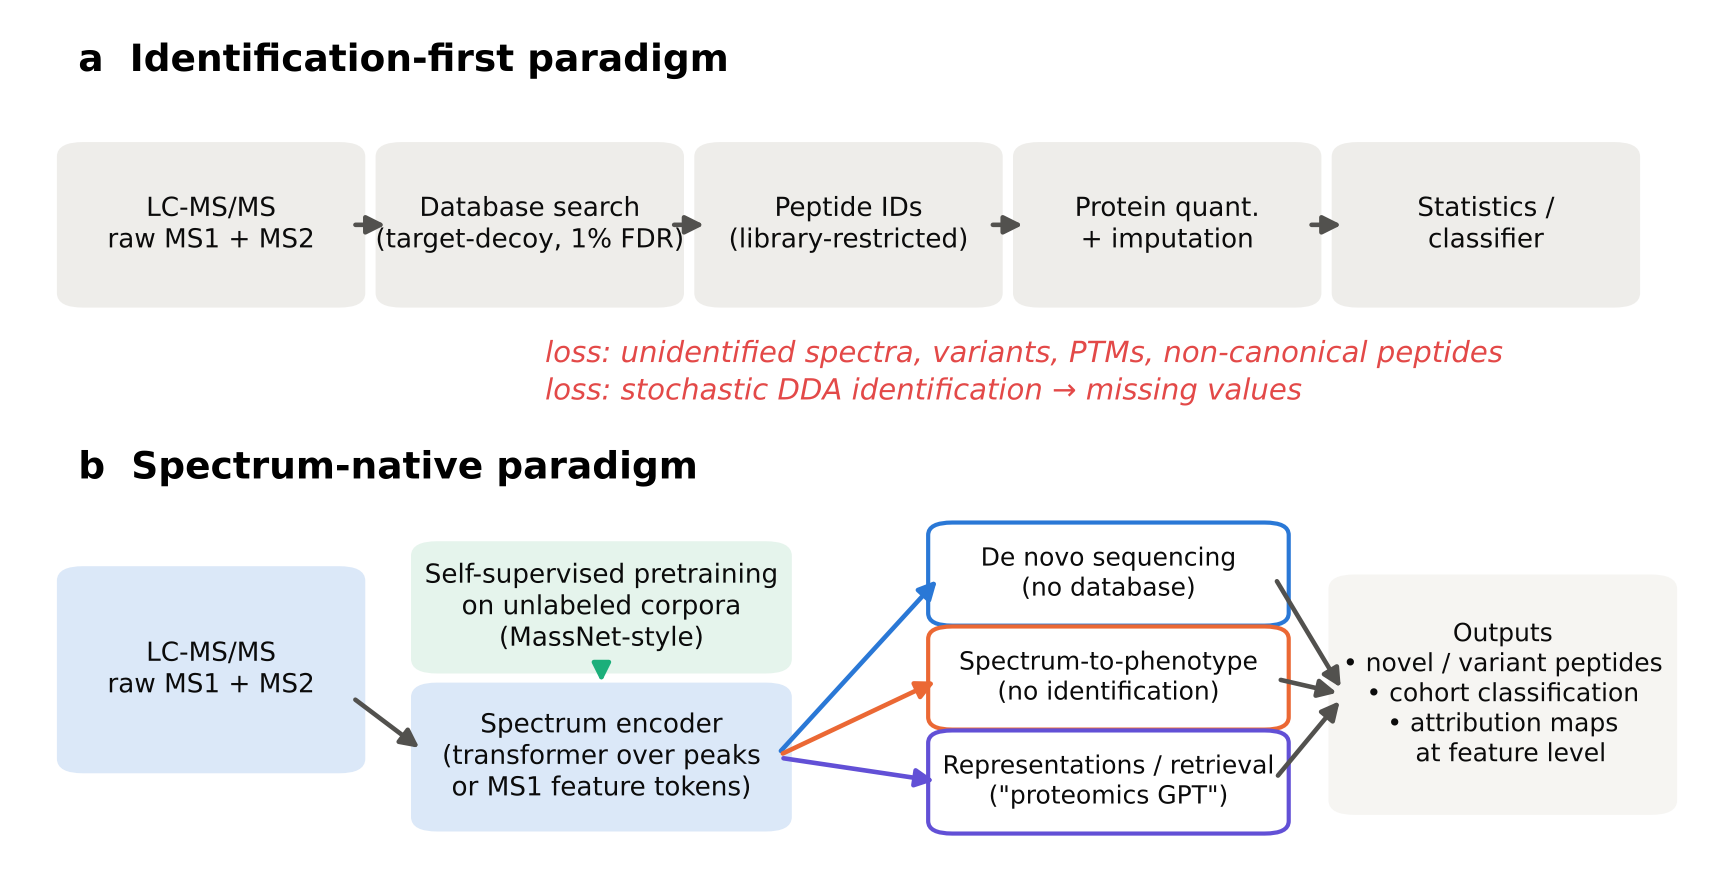
\includegraphics[width=1\textwidth,height=\textheight]{../figures/fig1_paradigm.png}
\caption{\textbf{Fig. 1. From identification-first to spectrum-native
proteomics.} (a) The classical workflow loses unidentified spectra,
variants, PTMs and non-canonical peptides at the search step, and
creates missing values through stochastic DDA identification. (b)
Spectrum-native models share an encoder that may be pretrained on
unlabeled corpora and support database-free sequencing,
identification-free phenotype prediction and representation learning.}
\end{figure}

\begin{figure}
\centering
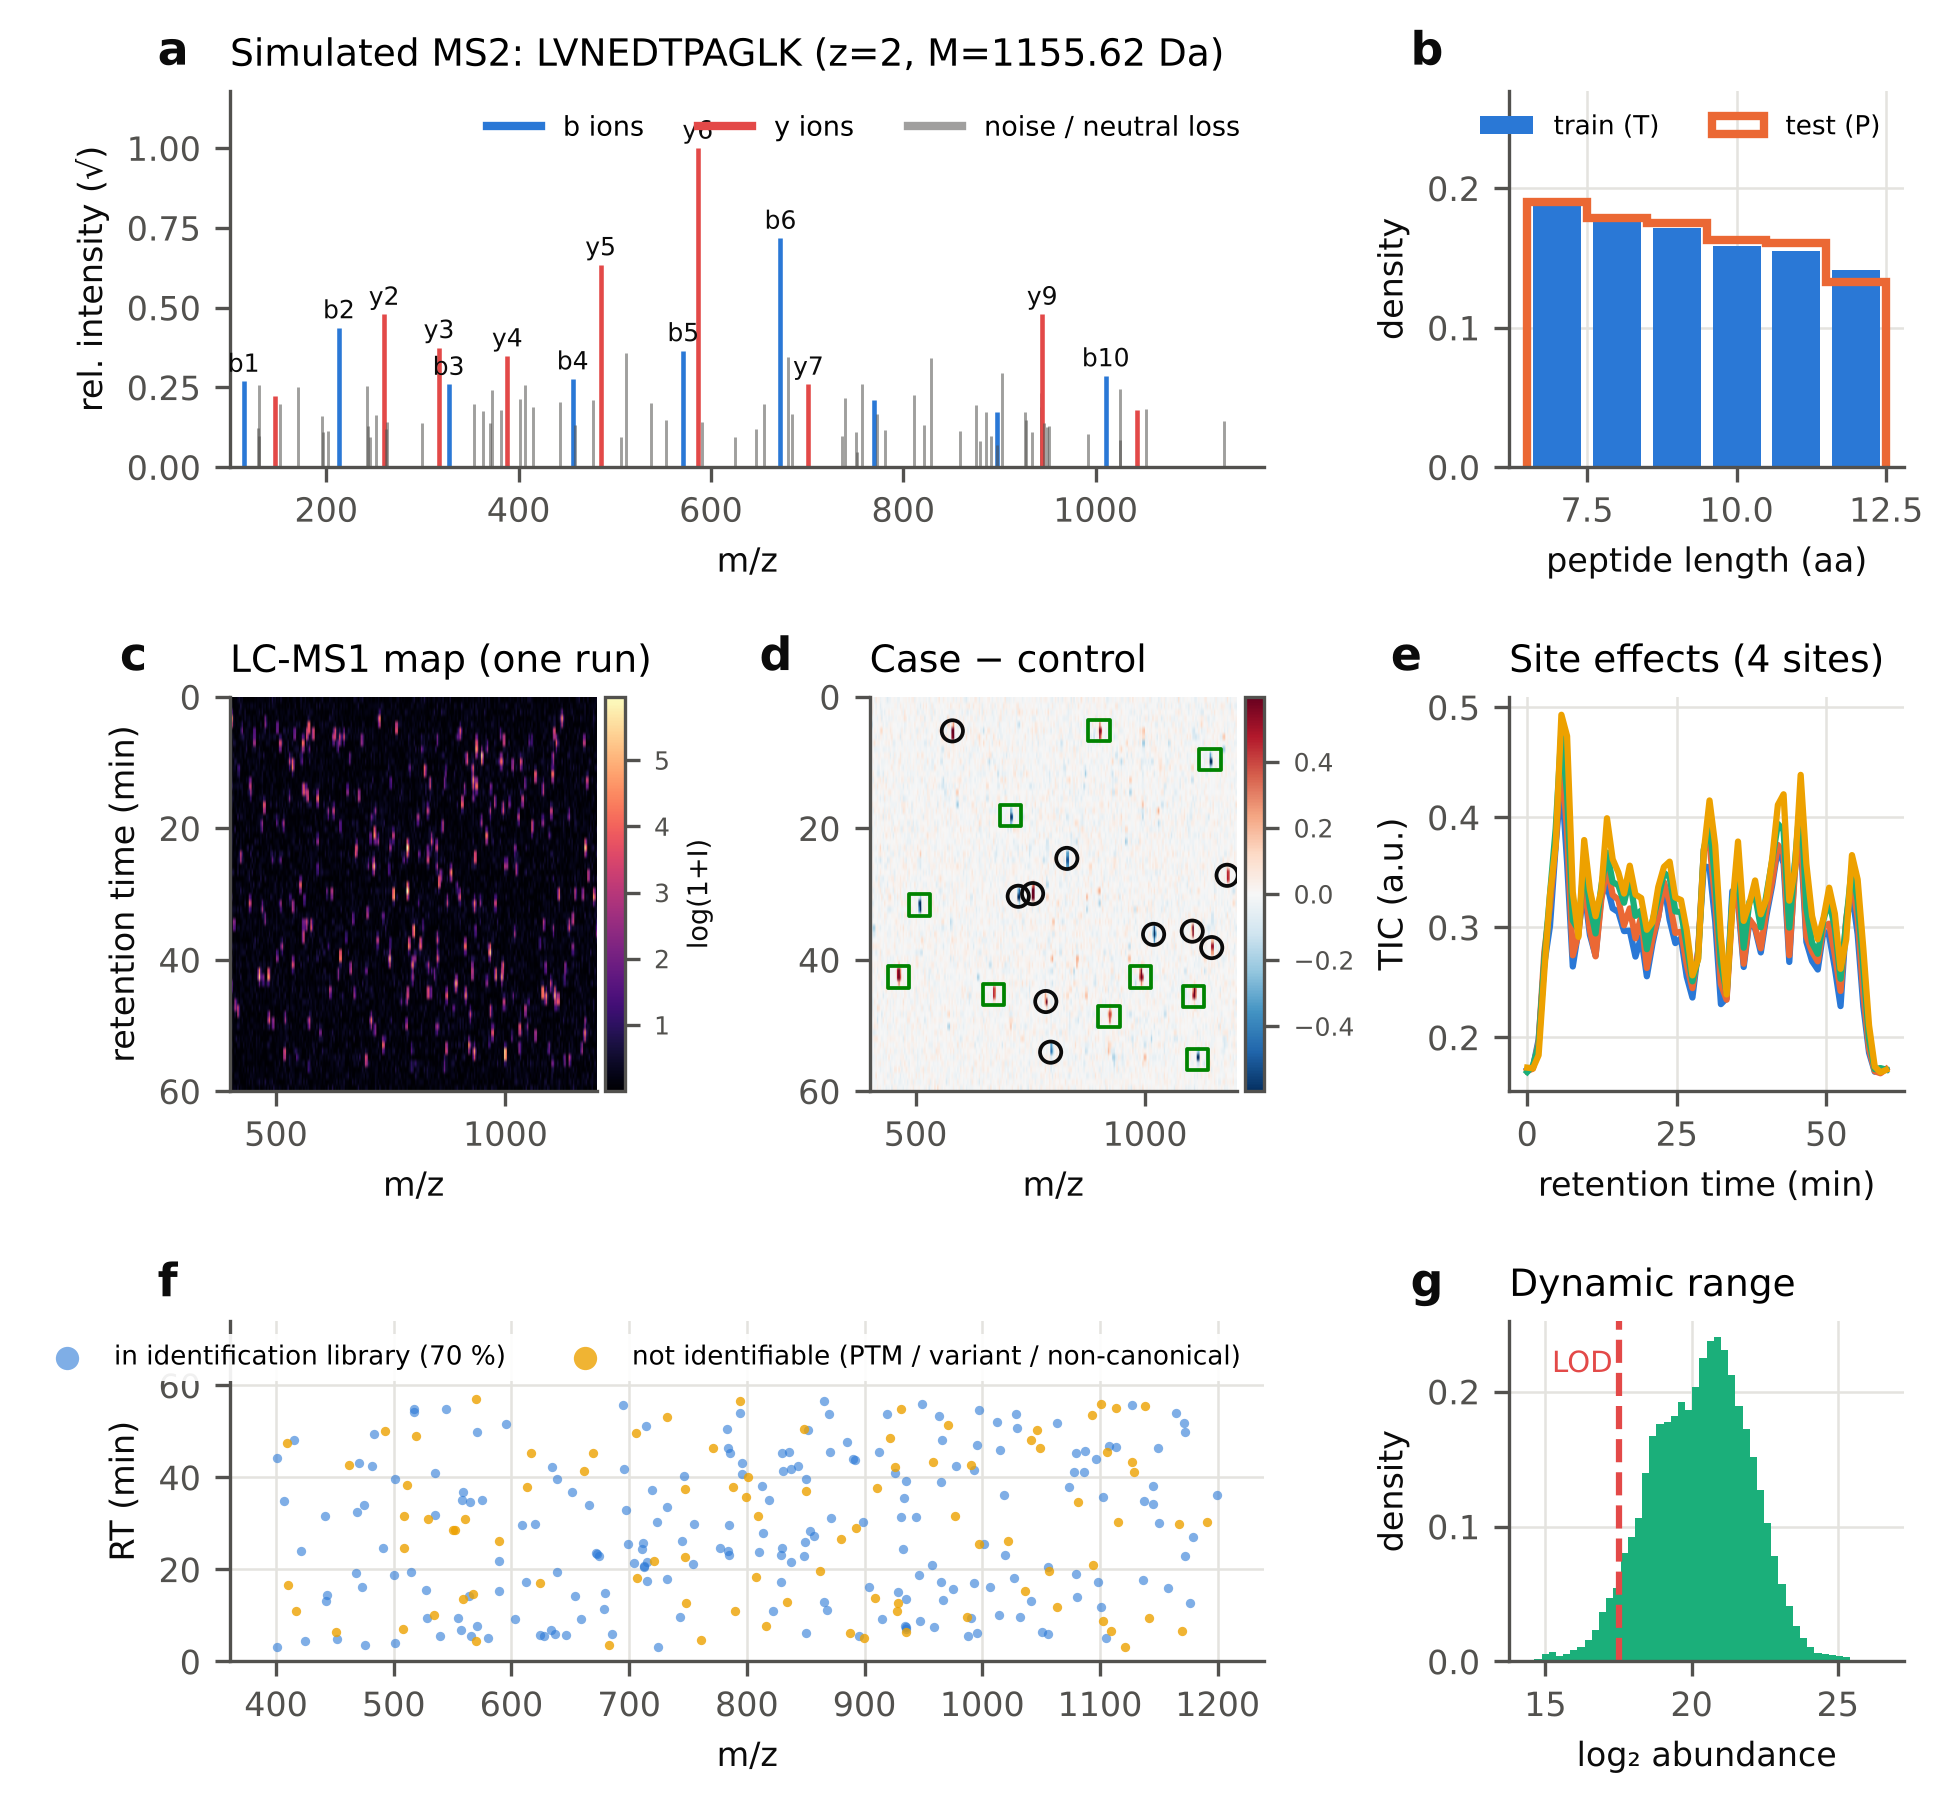
\includegraphics[width=1\textwidth,height=\textheight]{../figures/fig2_virtual_instrument.png}
\caption{\textbf{Fig. 2. The virtual instrument.} (a) Simulated MS2
spectrum of LVNEDTPAGLK with annotated b (blue) and y (red) ions; grey,
noise and neutral-loss peaks. (b) Peptide-length distributions of
training (proteome T) and test (proteome P) spectra. (c) Rendered LC-MS1
map of one run (64 RT × 256 m/z bins). (d) Mean case − control
difference map; circles, library biomarkers; squares, unidentifiable
biomarkers. (e) Total-ion chromatograms of the four acquisition sites.
(f) MS1 feature landscape coloured by identifiability. (g) Abundance
distribution and limit of detection (LOD).}
\end{figure}

\textbf{Table 1. Benchmark corpora generated by the virtual instrument.}

\begin{longtable}[]{@{}
  >{\raggedright\arraybackslash}p{(\columnwidth - 8\tabcolsep) * \real{0.2000}}
  >{\raggedright\arraybackslash}p{(\columnwidth - 8\tabcolsep) * \real{0.2000}}
  >{\raggedright\arraybackslash}p{(\columnwidth - 8\tabcolsep) * \real{0.2000}}
  >{\raggedright\arraybackslash}p{(\columnwidth - 8\tabcolsep) * \real{0.2000}}
  >{\raggedright\arraybackslash}p{(\columnwidth - 8\tabcolsep) * \real{0.2000}}@{}}
\toprule\noalign{}
\begin{minipage}[b]{\linewidth}\raggedright
Corpus / set
\end{minipage} & \begin{minipage}[b]{\linewidth}\raggedright
Source
\end{minipage} & \begin{minipage}[b]{\linewidth}\raggedright
Spectra
\end{minipage} & \begin{minipage}[b]{\linewidth}\raggedright
Unique peptides
\end{minipage} & \begin{minipage}[b]{\linewidth}\raggedright
Condition
\end{minipage} \\
\midrule\noalign{}
\endhead
\bottomrule\noalign{}
\endlastfoot
Training & proteome T (3,000 proteins) & 250,000 & 73,126 &
\emph{p}\textsubscript{obs} ∼ U(0.55, 0.95), λ ∼ U(10, 100) \\
Validation & proteome T & 2,000 & -- & \emph{p}\textsubscript{obs} =
0.80, λ = 40 \\
inDB & proteome P (in database) & 3,000 & 3,000 &
\emph{p}\textsubscript{obs} = 0.80, λ = 40 \\
SAAV & P + single AA variant & 1,500 & 1,500 &
\emph{p}\textsubscript{obs} = 0.80, λ = 40 \\
novel & proteome N (not in DB) & 1,500 & 1,500 &
\emph{p}\textsubscript{obs} = 0.80, λ = 40 \\
Robustness ×8 & proteome P & 8 × 1,000 & -- &
\emph{p}\textsubscript{obs} ∈ \{0.95, 0.80, 0.65, 0.50\}; λ ∈
\{10,40,100,200\} \\
Search database & proteome P targets (+Met-ox) & -- & 45,779 & + equal
number of reversed decoys \\
MS1 cohorts & 300 features, 4 sites & 800 unlabeled + 384 labelled + 500
test runs / seed & -- & 20 biomarkers, absolute log₂FC 0.26--0.44 \\
\end{longtable}

\textbf{Table 2. Model and training configurations.}

\begin{longtable}[]{@{}
  >{\raggedright\arraybackslash}p{(\columnwidth - 4\tabcolsep) * \real{0.3333}}
  >{\raggedright\arraybackslash}p{(\columnwidth - 4\tabcolsep) * \real{0.3333}}
  >{\raggedright\arraybackslash}p{(\columnwidth - 4\tabcolsep) * \real{0.3333}}@{}}
\toprule\noalign{}
\begin{minipage}[b]{\linewidth}\raggedright
Item
\end{minipage} & \begin{minipage}[b]{\linewidth}\raggedright
SpecNovo
\end{minipage} & \begin{minipage}[b]{\linewidth}\raggedright
FeatureFormer
\end{minipage} \\
\midrule\noalign{}
\endhead
\bottomrule\noalign{}
\endlastfoot
Input & ≤ 80 peaks (m/z, √I) + precursor (M, z) & 300 aligned MS1
features (value or missing) \\
Embedding & sinusoidal m/z (λ 10⁻³--10⁴ Da) + complementary m/z +
intensity & feature ID + 0.1·sin(m/z, RT) + value × w\_j (FT-style) \\
Encoder & 3 × pre-norm transformer, d = 128, 4 heads, FF 512 & 2 ×
pre-norm transformer, d = 64, 4 heads, FF 128 \\
Decoder / head & 3-layer autoregressive decoder + prefix/residual mass +
ion-evidence MLP (8→32→1) & {[}CLS{]} logit + zero-initialised additive
token evidence \\
Parameters & 1.44 M & 0.14 M \\
Objective & cross-entropy, label smoothing 0.05 & SSL: masked-intensity
MSE (30 \%); fine-tune: cross-entropy, smoothing 0.1 \\
Optimiser & AdamW, lr 5 × 10⁻⁴ (3 × 10⁻⁴ for evidence stage), cosine,
batch 128 & AdamW, one-cycle, lr 10⁻³ (head) / 2 × 10⁻⁴ (body), batch
32, 150 steps \\
Inference & beam K = 5, precursor-mass constraint 0.05 Da & single
forward pass \\
Hardware & 3 CPU threads; final model ≈ 1.45 h wall-clock (mass-aware +
evidence stages) & 1 CPU thread per seed \\
\end{longtable}

\begin{figure}
\centering
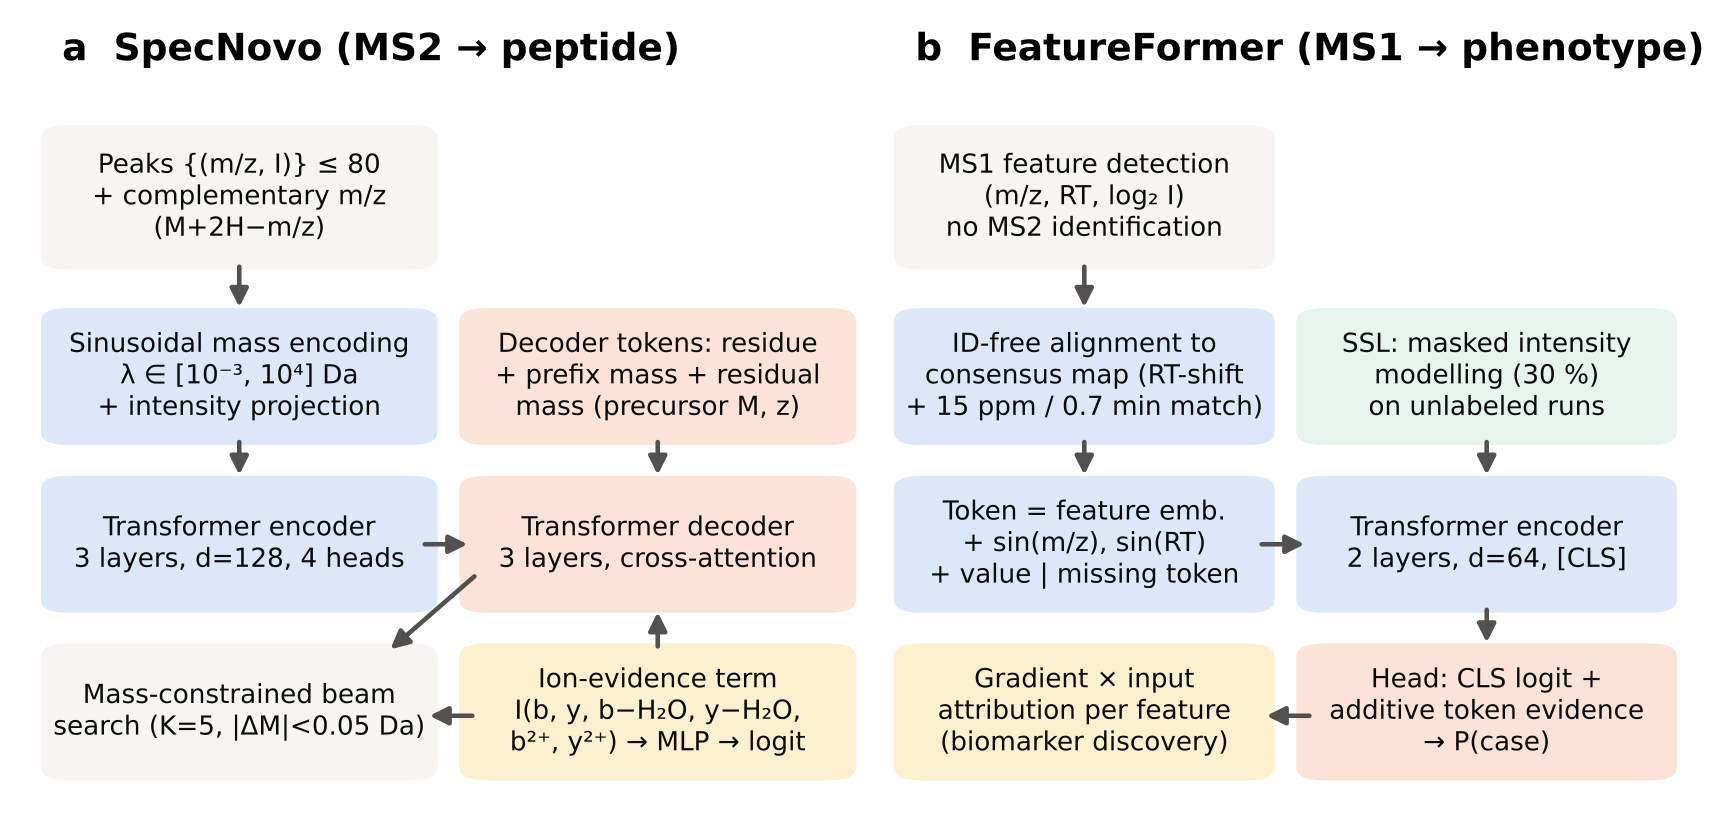
\includegraphics[width=1\textwidth,height=\textheight]{../figures/fig3_architecture.png}
\caption{\textbf{Fig. 3. Model architectures.} (a) SpecNovo encodes
peaks and their complementary masses, decodes residues conditioned on
prefix and residual mass, and adds a differentiable ion-evidence logit;
decoding is mass-constrained. (b) FeatureFormer tokenises
identification-free MS1 features, is pretrained by masked-intensity
modelling on unlabeled runs and fine-tuned for phenotype; gradient ×
input yields feature-level attributions.}
\end{figure}

\hypertarget{database-free-sequencing-recovers-peptides-that-database-search-cannot}{%
\subsection{Database-free sequencing recovers peptides that database
search
cannot}\label{database-free-sequencing-recovers-peptides-that-database-search-cannot}}

On canonical peptides, target--decoy database search was essentially
perfect: recall 0.999 at 1 \% FDR, with 0.03 \% false identifications
(Table 3, Fig. 4c). This is the regime for which identification-first
proteomics was designed. Introducing a single amino-acid variant, or
drawing peptides from a proteome absent from the database, reduced
database-search recall to 0.000 (Table 3). Target--decoy competition
correctly rejected the near-miss target matches, so no false
identifications passed 1 \% FDR; but every variant and novel peptide was
lost.

Both de novo methods were, as expected, insensitive to database
membership. SpecNovo recall was 0.416, 0.389 and 0.387, and
spectrum-graph recall 0.475, 0.475 and 0.468, on the canonical, SAAV and
novel sets respectively.

At full coverage the classical spectrum-graph algorithm had higher
peptide recall and amino-acid precision (0.834 vs 0.687 on inDB).
SpecNovo, however, produced better-ranked confidence scores, with
precision--coverage AUC of 0.663 vs 0.630 (Fig. 4b). Its precision was
higher whenever predictions were filtered by confidence:

\begin{longtable}[]{@{}lll@{}}
\toprule\noalign{}
Coverage (inDB) & SpecNovo precision & Spectrum-graph precision \\
\midrule\noalign{}
\endhead
\bottomrule\noalign{}
\endlastfoot
10 \% & 0.874 & 0.801 \\
25 \% & 0.787 & 0.716 \\
50 \% & 0.660 & 0.612 \\
\end{longtable}

The same held for SAAV spectra, where precision at 10 \% coverage was
0.905 vs 0.743. In practice, this is the regime that matters for
database-free discovery, where only high-confidence de novo calls are
followed up.

\textbf{Table 3. Database-dependent and database-free peptide
identification.}

\begin{longtable}[]{@{}
  >{\raggedright\arraybackslash}p{(\columnwidth - 12\tabcolsep) * \real{0.1429}}
  >{\raggedright\arraybackslash}p{(\columnwidth - 12\tabcolsep) * \real{0.1429}}
  >{\raggedright\arraybackslash}p{(\columnwidth - 12\tabcolsep) * \real{0.1429}}
  >{\raggedright\arraybackslash}p{(\columnwidth - 12\tabcolsep) * \real{0.1429}}
  >{\raggedright\arraybackslash}p{(\columnwidth - 12\tabcolsep) * \real{0.1429}}
  >{\raggedright\arraybackslash}p{(\columnwidth - 12\tabcolsep) * \real{0.1429}}
  >{\raggedright\arraybackslash}p{(\columnwidth - 12\tabcolsep) * \real{0.1429}}@{}}
\toprule\noalign{}
\begin{minipage}[b]{\linewidth}\raggedright
Test set
\end{minipage} & \begin{minipage}[b]{\linewidth}\raggedright
Method
\end{minipage} & \begin{minipage}[b]{\linewidth}\raggedright
AA precision
\end{minipage} & \begin{minipage}[b]{\linewidth}\raggedright
AA recall
\end{minipage} & \begin{minipage}[b]{\linewidth}\raggedright
Peptide recall
\end{minipage} & \begin{minipage}[b]{\linewidth}\raggedright
PR-AUC
\end{minipage} & \begin{minipage}[b]{\linewidth}\raggedright
False IDs (1 \% FDR)
\end{minipage} \\
\midrule\noalign{}
\endhead
\bottomrule\noalign{}
\endlastfoot
inDB & DB-search & -- & -- & 0.999 & -- & 0.000 \\
inDB & SpectrumGraph-DP & 0.834 & 0.876 & 0.475 & 0.630 & -- \\
inDB & SpecNovo & 0.687 & 0.698 & 0.416 & 0.663 & -- \\
SAAV & DB-search & -- & -- & 0.000 & -- & 0.000 \\
SAAV & SpectrumGraph-DP & 0.835 & 0.877 & 0.475 & 0.615 & -- \\
SAAV & SpecNovo & 0.670 & 0.684 & 0.389 & 0.646 & -- \\
novel & DB-search & -- & -- & 0.000 & -- & 0.000 \\
novel & SpectrumGraph-DP & 0.832 & 0.876 & 0.468 & 0.622 & -- \\
novel & SpecNovo & 0.670 & 0.684 & 0.387 & 0.634 & -- \\
\end{longtable}

\begin{figure}
\centering
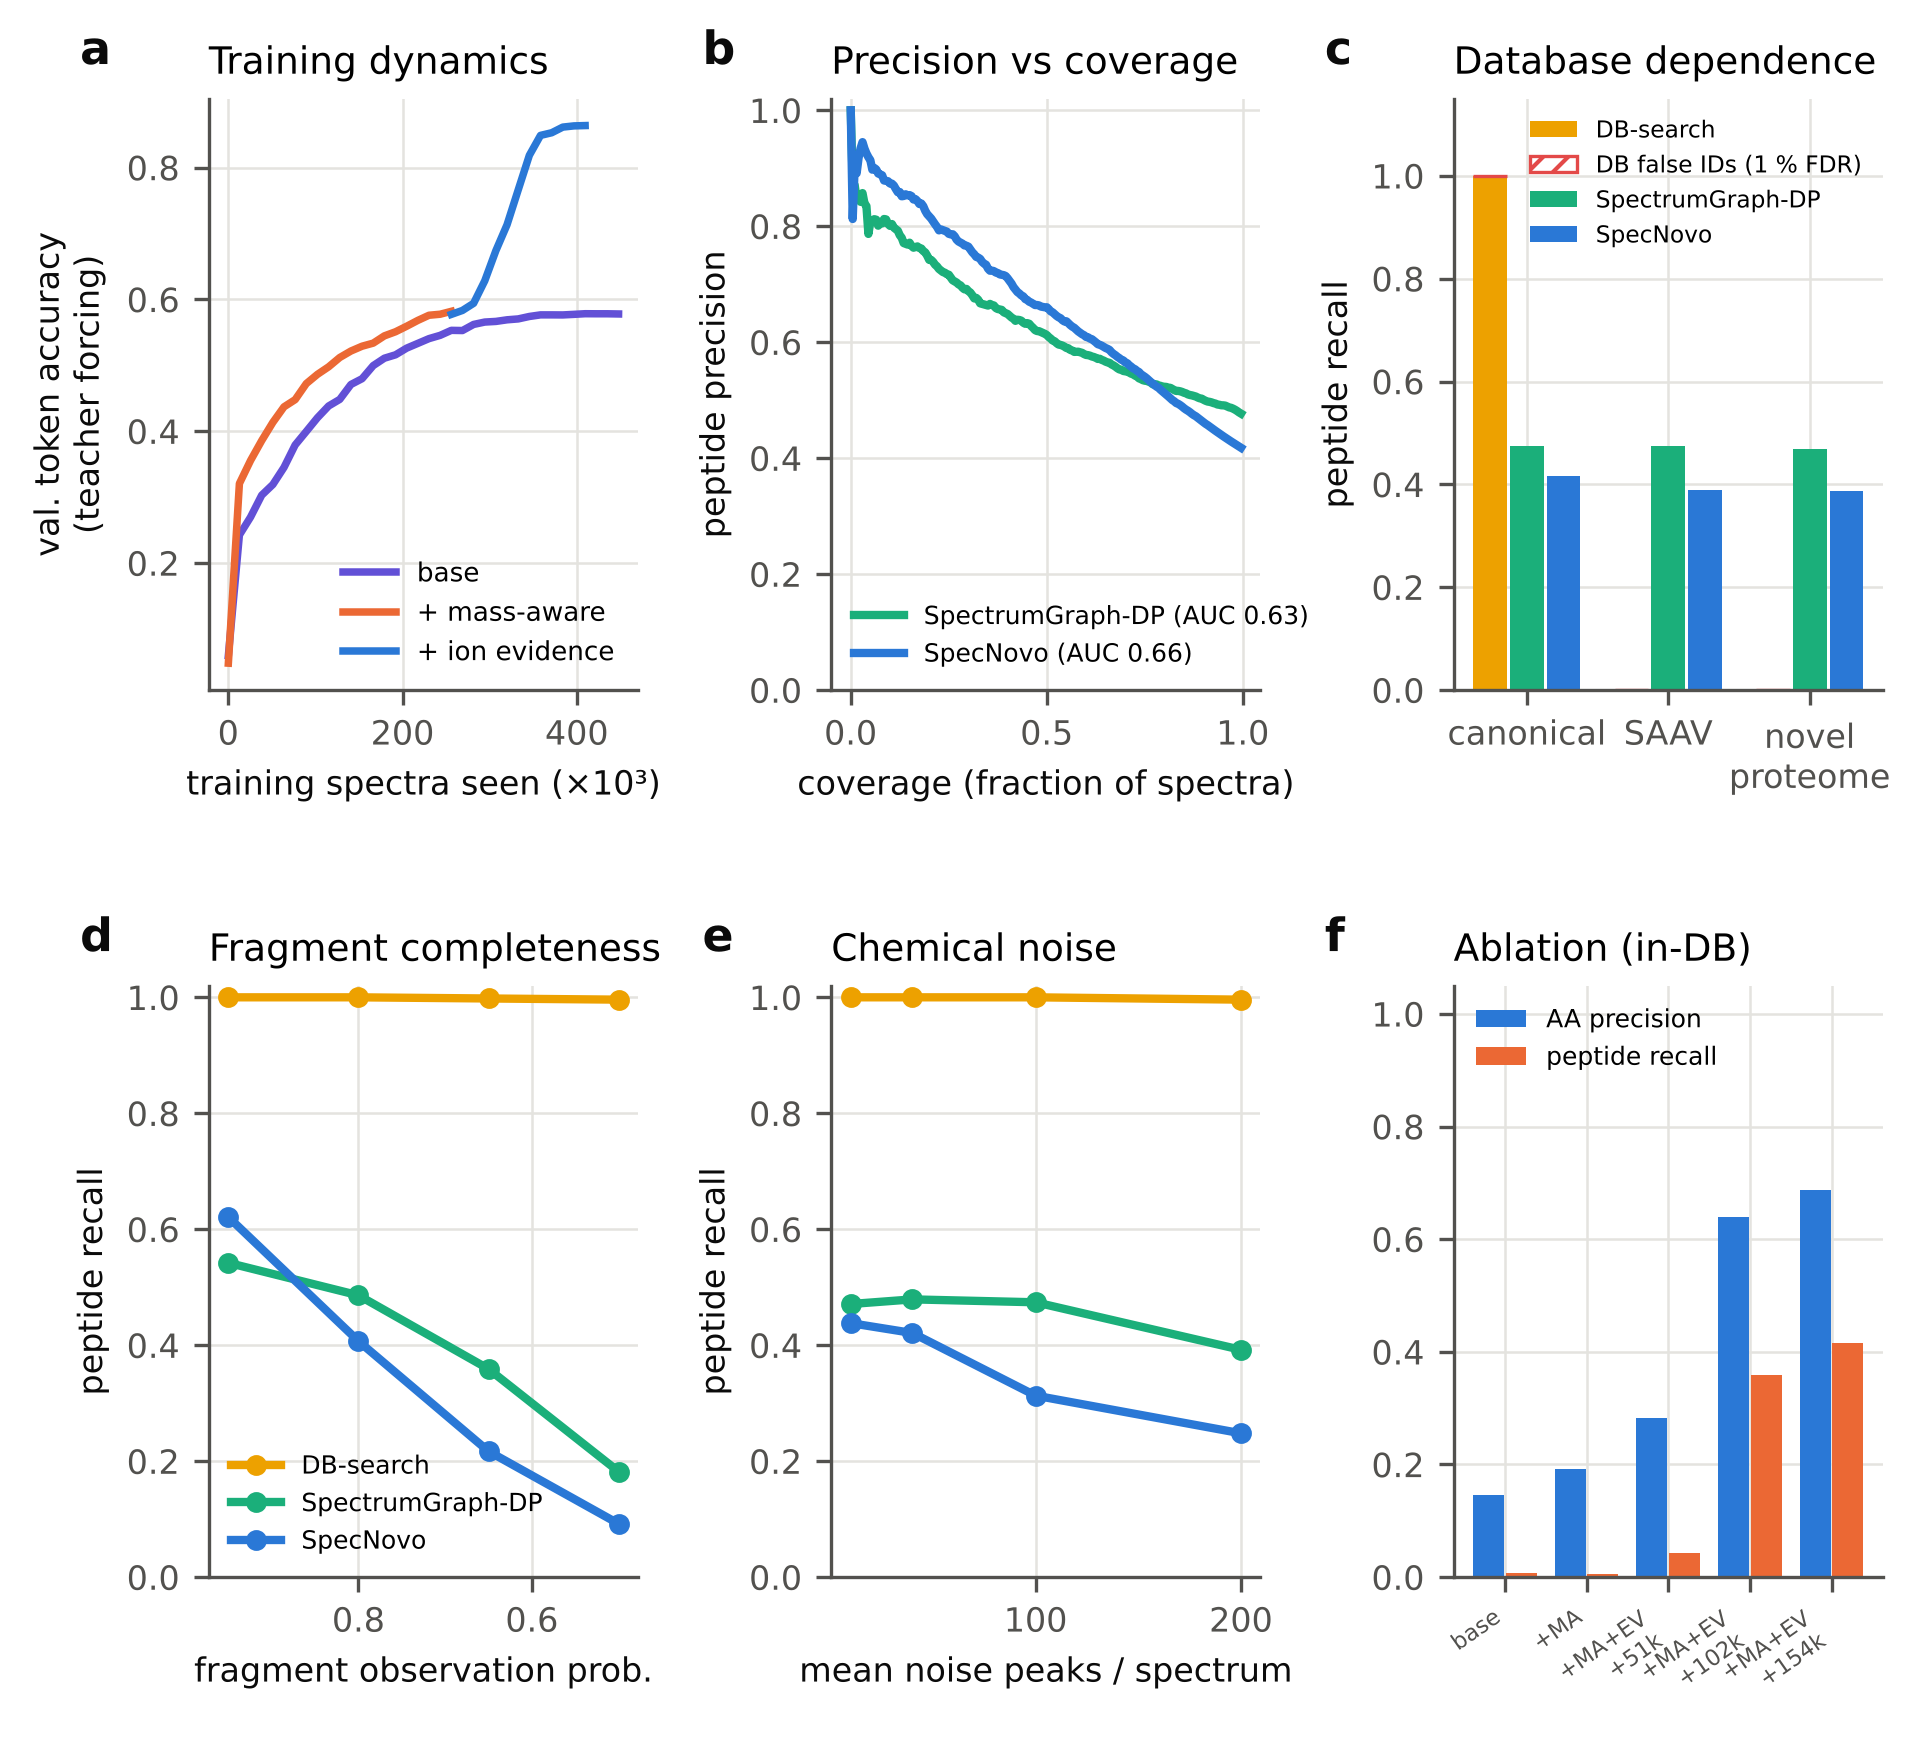
\includegraphics[width=1\textwidth,height=\textheight]{../figures/fig4_denovo.png}
\caption{\textbf{Fig. 4. De novo sequencing benchmark.} (a) Validation
token accuracy (teacher forcing) as a function of training spectra for
the base transformer, the mass-aware variant and the ion-evidence
variant (initialised from the mass-aware checkpoint). (b) Peptide
precision--coverage curves on inDB. (c) Peptide recall of database
search, spectrum-graph DP and SpecNovo on canonical, SAAV and
novel-proteome spectra; hatched, database false identifications at 1 \%
FDR. (d, e) Peptide recall versus fragment observation probability and
chemical-noise peaks. (f) Ablation: amino-acid precision and peptide
recall on inDB; MA, mass-aware; EV, ion evidence; +Nk, additional
training spectra.}
\end{figure}

\hypertarget{inductive-biases-not-capacity-determine-data-efficiency}{%
\subsection{Inductive biases, not capacity, determine data
efficiency}\label{inductive-biases-not-capacity-determine-data-efficiency}}

The ablation (Table 5, Fig. 4a,f) is the most instructive result of this
study. A standard Casanovo-style encoder--decoder reached a
teacher-forced validation token accuracy of 0.578 after 448k training
spectra. Under mass-constrained beam search, however, it achieved only
0.8 \% peptide recall and 0.146 amino-acid precision. Inspection of
greedy decodes showed that the model had learned the sequence prior
(C-terminal K/R, residue frequencies) but very little of the spectrum:
the decodes were plausible tryptic peptides that did not explain the
observed peaks.

Complementary-ion encoding and prefix/residual-mass conditioning
accelerated early learning (token accuracy 0.386 vs 0.303 at 38k
spectra) but saturated at the same level (0.582). Adding the
differentiable ion-evidence term broke this plateau within 1,200 further
optimisation steps. Token accuracy rose to 0.674, 0.849 and 0.864 after
51k, 102k and 154k additional spectra, and peptide recall rose to 4.3
\%, 35.9 \% and 41.6 \%. The total budget (410k spectra, ≈ 1.45 h of
wall-clock time on three CPU threads) is two orders of magnitude below
that used to train published de novo transformers (e.g., 30 M spectra
for Casanovo {[}9{]}). The ablation therefore quantifies how much a
physics-informed prior substitutes for data. It also explains why
repository-scale corpora are a precondition for purely data-driven
``proteomics GPTs''.

\textbf{Table 5. Ablation of SpecNovo inductive biases on the inDB test
set (beam K = 5).}

\begin{longtable}[]{@{}
  >{\raggedright\arraybackslash}p{(\columnwidth - 12\tabcolsep) * \real{0.1429}}
  >{\raggedright\arraybackslash}p{(\columnwidth - 12\tabcolsep) * \real{0.1429}}
  >{\raggedright\arraybackslash}p{(\columnwidth - 12\tabcolsep) * \real{0.1429}}
  >{\raggedright\arraybackslash}p{(\columnwidth - 12\tabcolsep) * \real{0.1429}}
  >{\raggedright\arraybackslash}p{(\columnwidth - 12\tabcolsep) * \real{0.1429}}
  >{\raggedright\arraybackslash}p{(\columnwidth - 12\tabcolsep) * \real{0.1429}}
  >{\raggedright\arraybackslash}p{(\columnwidth - 12\tabcolsep) * \real{0.1429}}@{}}
\toprule\noalign{}
\begin{minipage}[b]{\linewidth}\raggedright
Variant
\end{minipage} & \begin{minipage}[b]{\linewidth}\raggedright
Training spectra
\end{minipage} & \begin{minipage}[b]{\linewidth}\raggedright
Val. token acc. (TF)
\end{minipage} & \begin{minipage}[b]{\linewidth}\raggedright
AA precision
\end{minipage} & \begin{minipage}[b]{\linewidth}\raggedright
AA recall
\end{minipage} & \begin{minipage}[b]{\linewidth}\raggedright
Peptide recall
\end{minipage} & \begin{minipage}[b]{\linewidth}\raggedright
PR-AUC
\end{minipage} \\
\midrule\noalign{}
\endhead
\bottomrule\noalign{}
\endlastfoot
Base transformer & 448k & 0.578 & 0.146 & 0.216 & 0.008 & 0.036 \\
+ complementary ions \& prefix-mass decoding & 256k & 0.582 & 0.192 &
0.214 & 0.005 & 0.021 \\
+ ion-evidence term (+400 steps) & 307k & 0.674 & 0.282 & 0.305 & 0.043
& 0.123 \\
+ ion-evidence term (+800 steps) & 358k & 0.849 & 0.639 & 0.656 & 0.359
& 0.598 \\
+ ion-evidence term (+1,200 steps, final) & 410k & 0.864 & 0.687 & 0.698
& 0.416 & 0.663 \\
\end{longtable}

\hypertarget{robustness-where-classical-algorithms-still-win}{%
\subsection{Robustness: where classical algorithms still
win}\label{robustness-where-classical-algorithms-still-win}}

Fragment completeness was the dominant factor (Table 4, Fig. 4d). With
nearly complete ladders (\emph{p}\textsubscript{obs} = 0.95), SpecNovo
outperformed the spectrum graph: peptide recall 0.621 vs 0.542, PR-AUC
0.840 vs 0.693. Below \emph{p}\textsubscript{obs} ≈ 0.9 the ranking
reversed, and at \emph{p}\textsubscript{obs} = 0.5 SpecNovo recalled 9.2
\% of peptides against 18.2 \% for the spectrum graph. SpecNovo was also
more sensitive to chemical noise (Fig. 4e). From λ = 10 to 200 noise
peaks its recall fell from 0.438 to 0.248, while the spectrum graph fell
only from 0.471 to 0.392.

Database search was robust to both perturbations (≥ 0.996), confirming
that the hard part of de novo sequencing is the missing information, not
the spectrum quality per se. These results mark the current limits of
small spectrum-native models. More training data that covers sparse and
noisy spectra, or hybrid models that combine learned scoring with
exhaustive graph search, are the obvious next steps.

\textbf{Table 4. Robustness to fragment completeness and chemical noise
(1,000 spectra per condition).}

\begin{longtable}[]{@{}
  >{\raggedright\arraybackslash}p{(\columnwidth - 14\tabcolsep) * \real{0.1250}}
  >{\raggedright\arraybackslash}p{(\columnwidth - 14\tabcolsep) * \real{0.1250}}
  >{\raggedright\arraybackslash}p{(\columnwidth - 14\tabcolsep) * \real{0.1250}}
  >{\raggedright\arraybackslash}p{(\columnwidth - 14\tabcolsep) * \real{0.1250}}
  >{\raggedright\arraybackslash}p{(\columnwidth - 14\tabcolsep) * \real{0.1250}}
  >{\raggedright\arraybackslash}p{(\columnwidth - 14\tabcolsep) * \real{0.1250}}
  >{\raggedright\arraybackslash}p{(\columnwidth - 14\tabcolsep) * \real{0.1250}}
  >{\raggedright\arraybackslash}p{(\columnwidth - 14\tabcolsep) * \real{0.1250}}@{}}
\toprule\noalign{}
\begin{minipage}[b]{\linewidth}\raggedright
Condition
\end{minipage} & \begin{minipage}[b]{\linewidth}\raggedright
DB-search pep. recall
\end{minipage} & \begin{minipage}[b]{\linewidth}\raggedright
SpectrumGraph-DP pep. recall
\end{minipage} & \begin{minipage}[b]{\linewidth}\raggedright
SpecNovo pep. recall
\end{minipage} & \begin{minipage}[b]{\linewidth}\raggedright
DP AA prec.
\end{minipage} & \begin{minipage}[b]{\linewidth}\raggedright
SpecNovo AA prec.
\end{minipage} & \begin{minipage}[b]{\linewidth}\raggedright
DP PR-AUC
\end{minipage} & \begin{minipage}[b]{\linewidth}\raggedright
SpecNovo PR-AUC
\end{minipage} \\
\midrule\noalign{}
\endhead
\bottomrule\noalign{}
\endlastfoot
\emph{p}\textsubscript{obs} = 0.95 & 1.000 & 0.542 & 0.621 & 0.865 &
0.808 & 0.693 & 0.840 \\
\emph{p}\textsubscript{obs} = 0.80 & 1.000 & 0.486 & 0.407 & 0.841 &
0.679 & 0.623 & 0.640 \\
\emph{p}\textsubscript{obs} = 0.65 & 0.998 & 0.359 & 0.217 & 0.776 &
0.533 & 0.504 & 0.440 \\
\emph{p}\textsubscript{obs} = 0.50 & 0.996 & 0.182 & 0.092 & 0.655 &
0.393 & 0.312 & 0.216 \\
λ = 10 & 1.000 & 0.471 & 0.438 & 0.844 & 0.707 & 0.619 & 0.669 \\
λ = 40 & 1.000 & 0.479 & 0.421 & 0.836 & 0.673 & 0.641 & 0.686 \\
λ = 100 & 1.000 & 0.474 & 0.313 & 0.833 & 0.625 & 0.620 & 0.535 \\
λ = 200 & 0.996 & 0.392 & 0.248 & 0.784 & 0.526 & 0.540 & 0.495 \\
\end{longtable}

\hypertarget{learned-representations-and-peak-level-attribution}{%
\subsection{Learned representations and peak-level
attribution}\label{learned-representations-and-peak-level-attribution}}

We tested whether the SpecNovo encoder learns peptide identity without
being trained to do so. We generated 12 independent noisy replicate
spectra for each of 40 test peptides (\emph{p}\textsubscript{obs} =
0.75, λ = 60) and compared mean-pooled encoder embeddings with 0.5 Da
binned spectra (Fig. 5a--c, Table 8).

The encoder embedding grouped replicates more compactly: cosine
silhouette 0.273 vs 0.222. Its top-1 replicate retrieval (0.908) was
slightly below that of binned spectra (0.996). In simulation, replicate
spectra share exact fragment m/z values, which favours binned matching;
on real data with calibration drift, learned embeddings such as GLEAMS
{[}19{]} are expected to have the advantage.

Gradient × input attribution showed that SpecNovo bases its predictions
on genuine fragment ions (Fig. 5d,e). Annotated b/y-family ions carried
42.2 \% of the total intensity but received 80.0 \% of the attribution
mass, and attribution exceeded the intensity share in 299 of 300
spectra. The model therefore actively down-weights noise peaks, an
interpretable behaviour that classical intensity-weighted scores do not
provide.

\begin{figure}
\centering
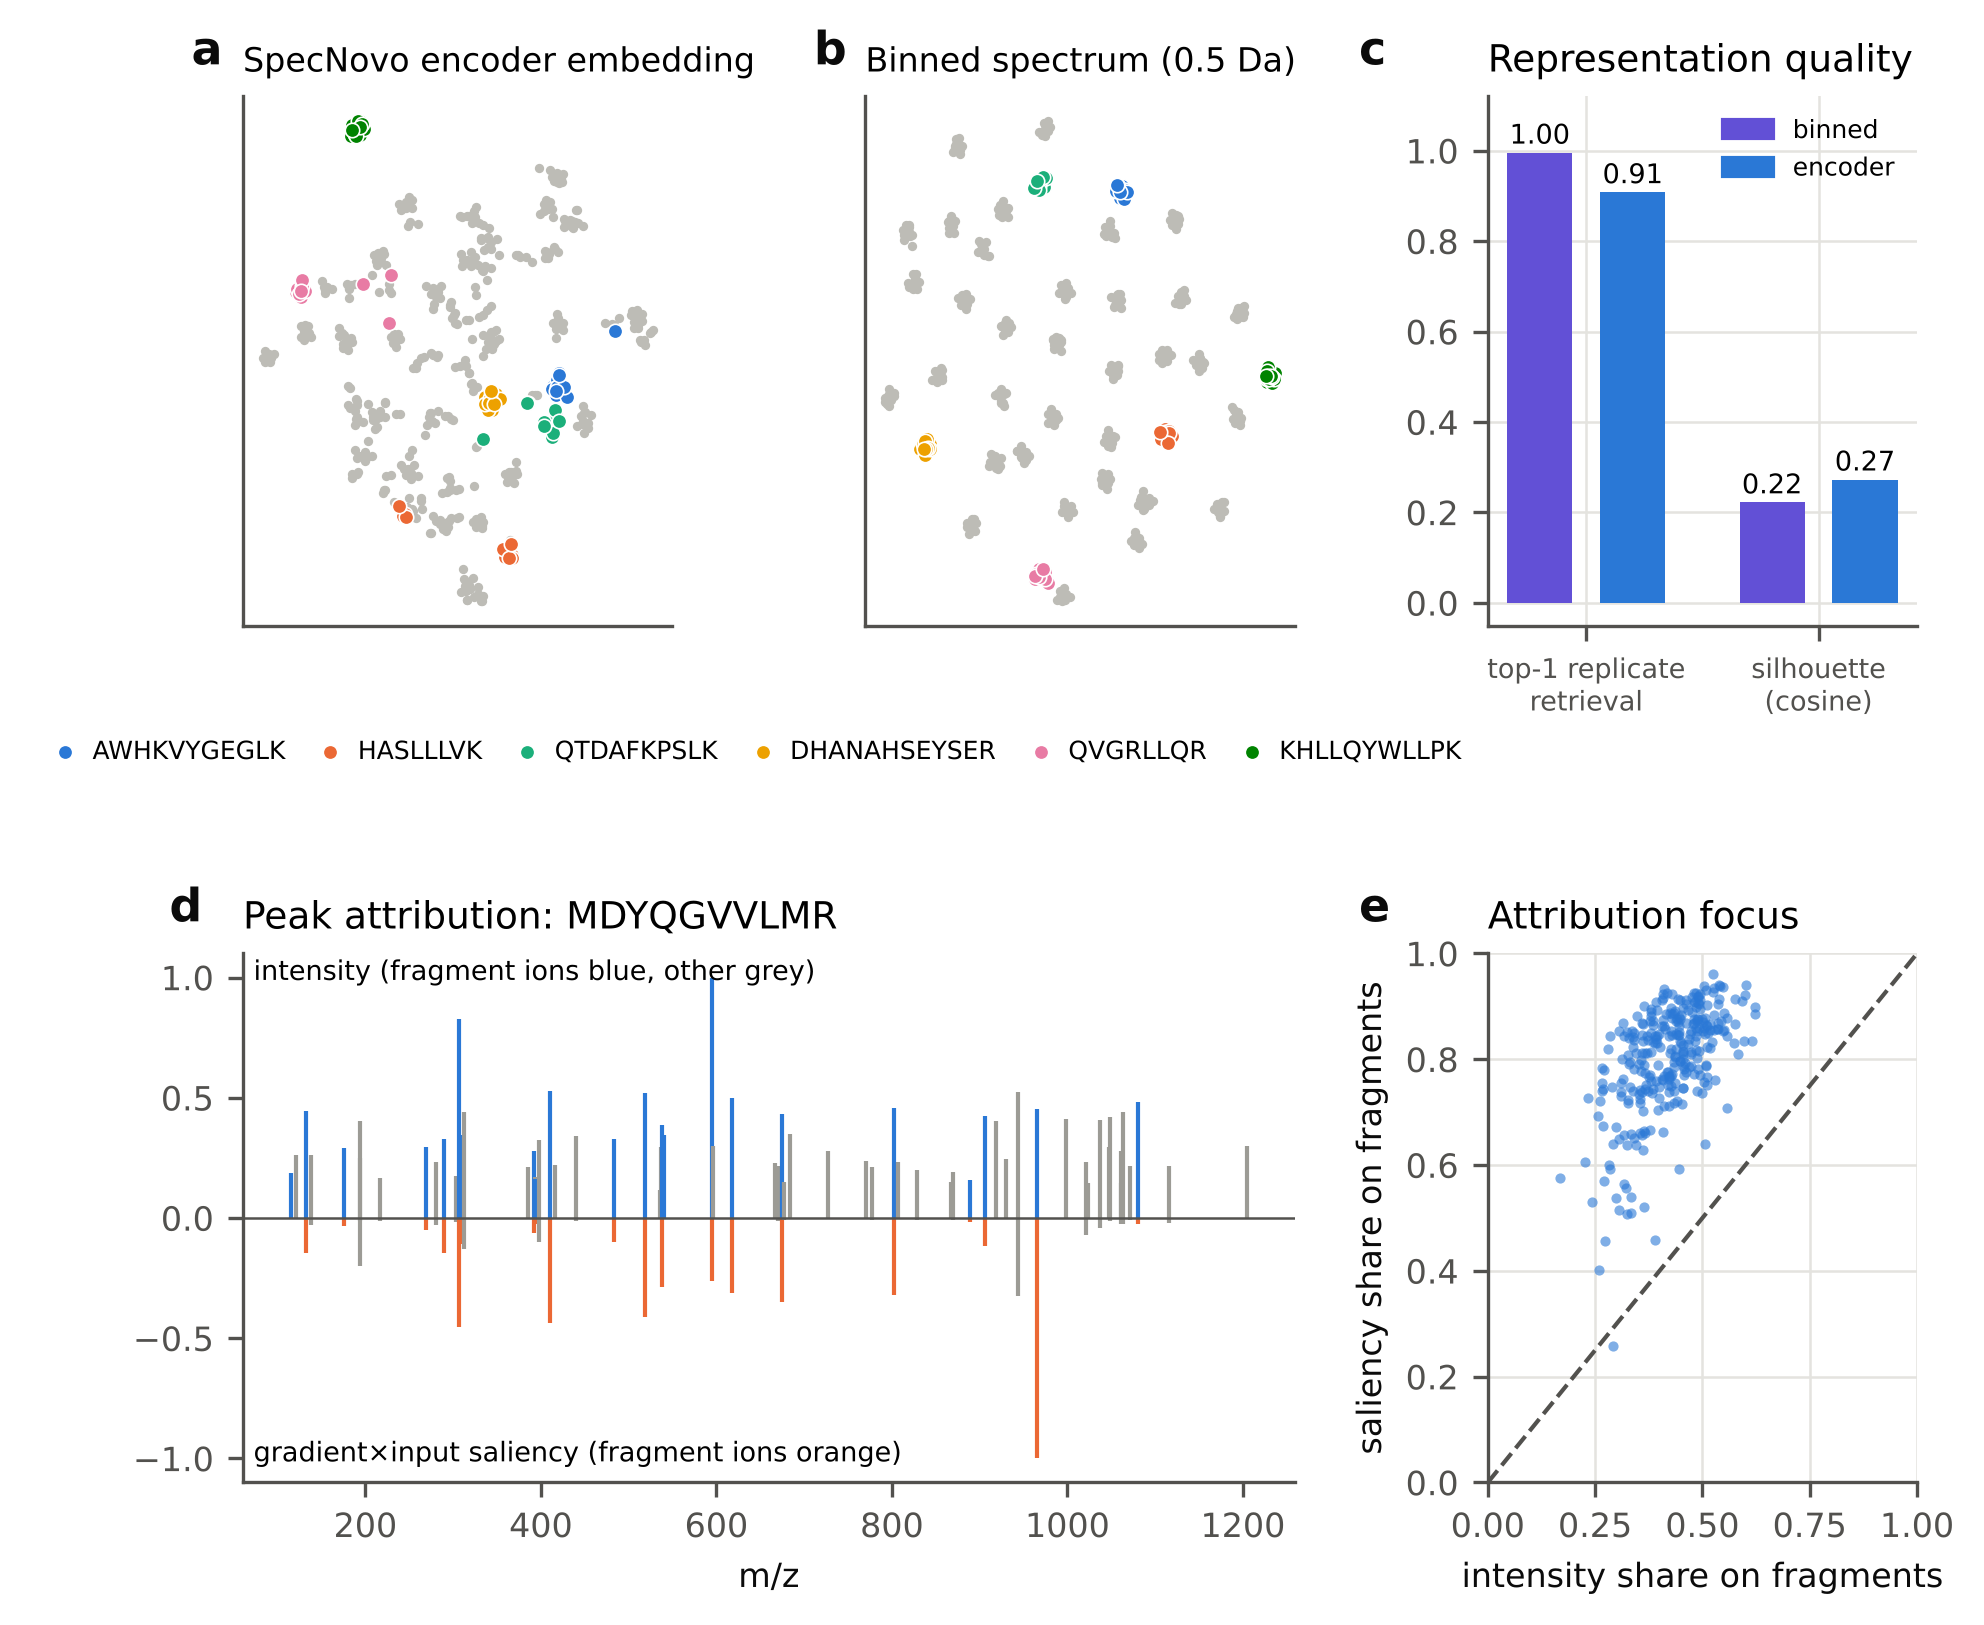
\includegraphics[width=1\textwidth,height=\textheight]{../figures/fig5_representation.png}
\caption{\textbf{Fig. 5. Representations and interpretability of
SpecNovo.} (a, b) t-SNE of 480 replicate spectra (40 peptides × 12)
using encoder embeddings (a) or binned spectra (b); six peptides
highlighted. (c) Top-1 replicate retrieval and cosine silhouette. (d)
Example spectrum: intensity (top; fragment ions blue) and gradient ×
input saliency (bottom; fragment ions orange). (e) Saliency share versus
intensity share on annotated fragment ions for 300 inDB spectra; dashed
line, identity.}
\end{figure}

\textbf{Table 8. Representation quality, interpretability and compute.}

\begin{longtable}[]{@{}
  >{\raggedright\arraybackslash}p{(\columnwidth - 4\tabcolsep) * \real{0.3333}}
  >{\raggedright\arraybackslash}p{(\columnwidth - 4\tabcolsep) * \real{0.3333}}
  >{\raggedright\arraybackslash}p{(\columnwidth - 4\tabcolsep) * \real{0.3333}}@{}}
\toprule\noalign{}
\begin{minipage}[b]{\linewidth}\raggedright
Analysis
\end{minipage} & \begin{minipage}[b]{\linewidth}\raggedright
Metric
\end{minipage} & \begin{minipage}[b]{\linewidth}\raggedright
Value
\end{minipage} \\
\midrule\noalign{}
\endhead
\bottomrule\noalign{}
\endlastfoot
Replicate retrieval (40 peptides × 12 spectra) & top-1 accuracy, encoder
embedding & 0.908 \\
& top-1 accuracy, binned spectrum (0.5 Da) & 0.996 \\
& silhouette (cosine), encoder & 0.273 \\
& silhouette (cosine), binned & 0.222 \\
Peak attribution (300 inDB spectra) & mean saliency share on annotated
fragment ions & 0.800 \\
& mean intensity share on annotated fragment ions & 0.422 \\
Inference cost & CPU seconds per 1,000 spectra (beam K=5, 2 threads) &
155 \\
Feature attribution (seed 0, n = 384) & AUROC of abs(grad × input) for
true biomarkers & 0.622 \\
& AUROC of Welch t-test −log10 p (ID-free matrix) & 1.000 \\
\end{longtable}

\hypertarget{spectrum-to-phenotype-removing-the-identification-bottleneck}{%
\subsection{Spectrum-to-phenotype: removing the identification
bottleneck}\label{spectrum-to-phenotype-removing-the-identification-bottleneck}}

The same theme dominated the MS1 experiments, at the cohort level (Table
6, Fig. 6). With half of the biomarkers unidentifiable, the
identification-first pipeline reached AUROC 0.558 with 24 labelled runs
and 0.672 with 384 (Fig. 6a). Two losses compound here: unidentified
biomarkers, and 25 \% missing values from stochastic DDA identification,
which minimum-value imputation turns into noise.

Match-between-runs (MBR) recovered the missing-value loss but not the
unidentified biomarkers (0.932 at n = 192). The identification-free
linear model, which uses all aligned features, was best at every label
budget: 0.820 at n = 24, 0.975 at n = 192 and 0.981 at n = 384. The
ProFormer-style FeatureFormer improved substantially on
identification-first statistics (0.767 vs 0.648 at n = 192; 0.802 vs
0.672 at n = 384). At these sample sizes it did not reach the
identification-free linear model, because the simulated phenotype signal
is additive and linear models are near-optimal for it.

Self-supervised masked-intensity pretraining on 800 unlabeled runs did
not improve in-distribution accuracy (0.714 vs 0.767 at n = 192). It did
improve transfer to an unseen acquisition site: leave-one-site-out AUROC
rose from 0.651 ± 0.087 to 0.728 ± 0.054, with lower variance (Fig. 6b).
Identification-free features also transferred best overall (0.986 ±
0.012), because ID-free RT-shift alignment absorbs site-specific
chromatographic drift.

\textbf{Table 6. Spectrum-to-phenotype AUROC (mean ± s.d. over three
seeds; 500 test runs; 50 \% of biomarkers unidentifiable).}

\begin{longtable}[]{@{}
  >{\raggedright\arraybackslash}p{(\columnwidth - 12\tabcolsep) * \real{0.1429}}
  >{\raggedright\arraybackslash}p{(\columnwidth - 12\tabcolsep) * \real{0.1429}}
  >{\raggedright\arraybackslash}p{(\columnwidth - 12\tabcolsep) * \real{0.1429}}
  >{\raggedright\arraybackslash}p{(\columnwidth - 12\tabcolsep) * \real{0.1429}}
  >{\raggedright\arraybackslash}p{(\columnwidth - 12\tabcolsep) * \real{0.1429}}
  >{\raggedright\arraybackslash}p{(\columnwidth - 12\tabcolsep) * \real{0.1429}}
  >{\raggedright\arraybackslash}p{(\columnwidth - 12\tabcolsep) * \real{0.1429}}@{}}
\toprule\noalign{}
\begin{minipage}[b]{\linewidth}\raggedright
Method
\end{minipage} & \begin{minipage}[b]{\linewidth}\raggedright
n = 24
\end{minipage} & \begin{minipage}[b]{\linewidth}\raggedright
n = 48
\end{minipage} & \begin{minipage}[b]{\linewidth}\raggedright
n = 96
\end{minipage} & \begin{minipage}[b]{\linewidth}\raggedright
n = 192
\end{minipage} & \begin{minipage}[b]{\linewidth}\raggedright
n = 384
\end{minipage} & \begin{minipage}[b]{\linewidth}\raggedright
LOSO (unseen site)
\end{minipage} \\
\midrule\noalign{}
\endhead
\bottomrule\noalign{}
\endlastfoot
ID-first-LR & 0.558 ± 0.050 & 0.587 ± 0.034 & 0.606 ± 0.007 & 0.648 ±
0.013 & 0.672 ± 0.040 & 0.627 ± 0.034 \\
ID-first+MBR-LR & 0.660 ± 0.070 & 0.818 ± 0.031 & 0.864 ± 0.005 & 0.932
± 0.020 & 0.945 ± 0.021 & 0.942 ± 0.019 \\
ID-free-LR & 0.820 ± 0.046 & 0.903 ± 0.003 & 0.942 ± 0.017 & 0.975 ±
0.015 & 0.981 ± 0.015 & 0.986 ± 0.012 \\
FeatureFormer & 0.661 ± 0.041 & 0.695 ± 0.023 & 0.693 ± 0.044 & 0.767 ±
0.037 & 0.802 ± 0.018 & 0.651 ± 0.087 \\
FeatureFormer+SSL & 0.593 ± 0.026 & 0.652 ± 0.042 & 0.674 ± 0.020 &
0.714 ± 0.015 & 0.737 ± 0.025 & 0.728 ± 0.054 \\
\end{longtable}

\begin{figure}
\centering
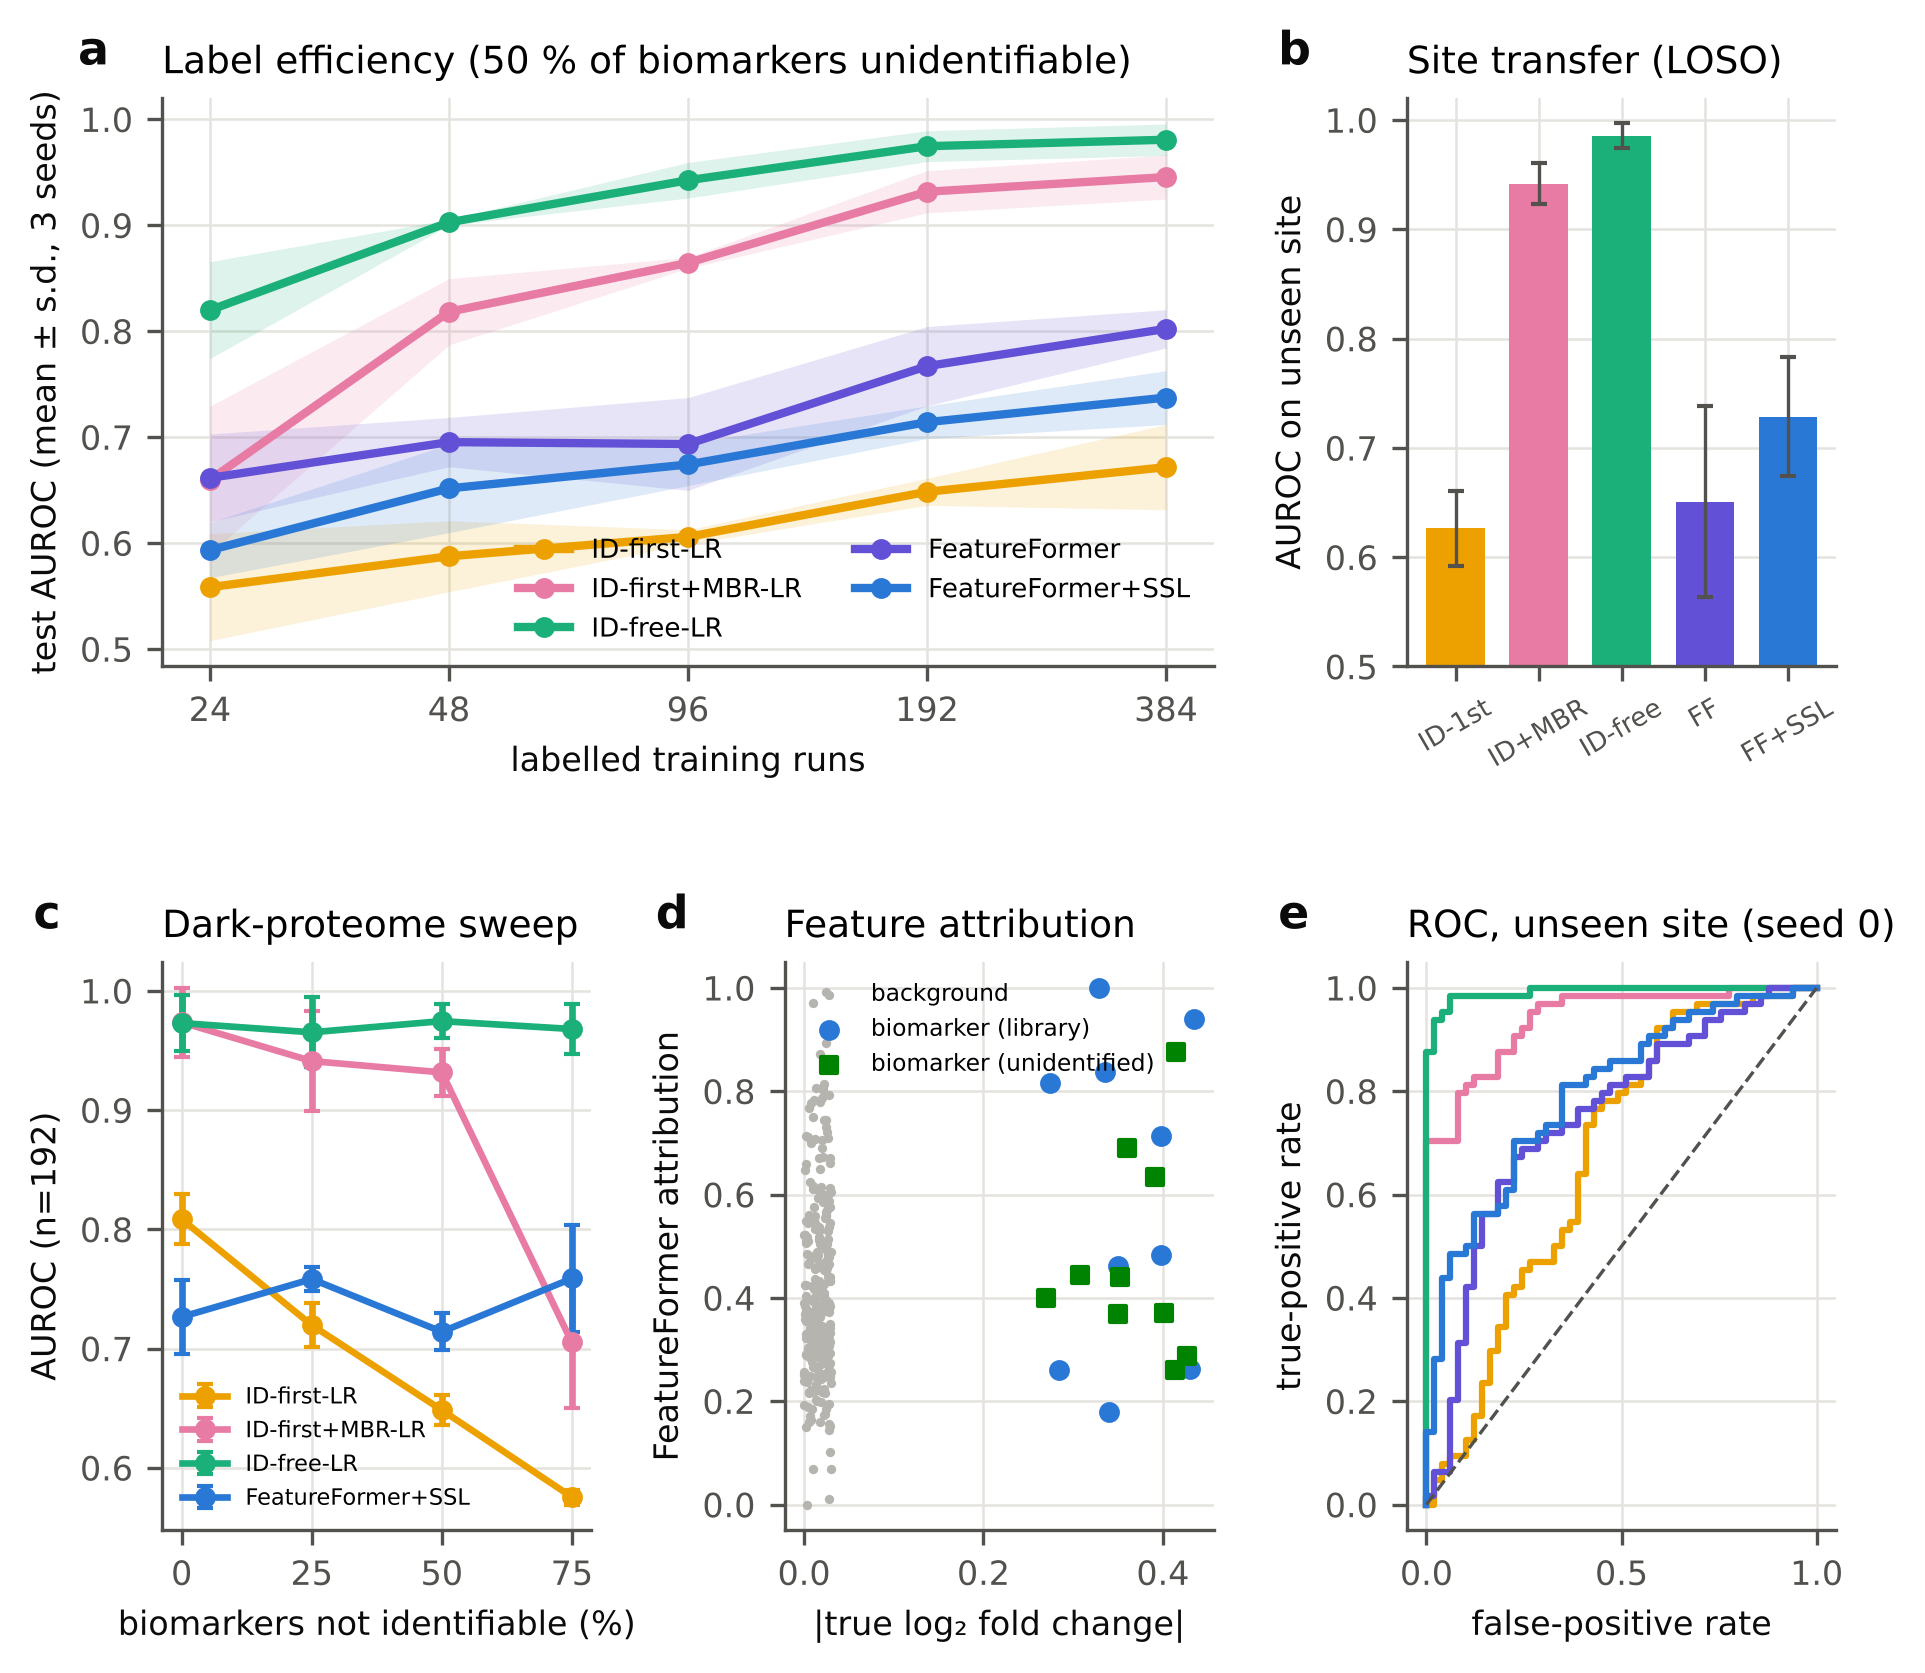
\includegraphics[width=1\textwidth,height=\textheight]{../figures/fig6_phenotype.png}
\caption{\textbf{Fig. 6. Spectrum-to-phenotype benchmark.} (a) Test
AUROC versus number of labelled runs (mean ± s.d., three seeds; 50 \% of
biomarkers unidentifiable). (b) Leave-one-site-out AUROC on an unseen
acquisition site. (c) AUROC (n = 192) versus fraction of biomarkers not
identifiable by MS2 search. (d) FeatureFormer gradient × input
attribution versus true effect size; library (circles) and
unidentifiable (squares) biomarkers. (e) ROC curves on the unseen site
(seed 0; colours as in a).}
\end{figure}

\hypertarget{the-dark-proteome-sweep-quantifies-information-loss}{%
\subsection{The dark-proteome sweep quantifies information
loss}\label{the-dark-proteome-sweep-quantifies-information-loss}}

Varying the fraction of unidentifiable biomarkers from 0 \% to 75 \%
separated the pipelines cleanly (Table 7, Fig. 6c). Identification-free
linear models were invariant to identifiability (0.973 → 0.968).
Identification-first AUROC declined monotonically (0.808 → 0.575),
approaching chance once three quarters of the biomarkers were dark. MBR
matched identification-free performance while most biomarkers were
identifiable (0.973 at 0 \%) but collapsed at 75 \% (0.705 ± 0.055).
FeatureFormer+SSL was likewise invariant to identifiability
(0.714--0.759), confirming that it uses unidentified signal, but it
remained limited by sample size.

Feature attribution recovered true biomarkers above chance (AUROC
0.622), including unidentifiable ones (Fig. 6d). However, a Welch t-test
on identification-free features ranked all 20 biomarkers above all
background features (AUROC 1.000). For biomarker \emph{discovery} in
additive settings, simple statistics on identification-free features
therefore remain the reference against which deep attribution must be
judged.

\textbf{Table 7. AUROC (n = 192) as a function of the fraction of
biomarkers that are not identifiable by MS2 database search.}

\begin{longtable}[]{@{}
  >{\raggedright\arraybackslash}p{(\columnwidth - 8\tabcolsep) * \real{0.2000}}
  >{\raggedright\arraybackslash}p{(\columnwidth - 8\tabcolsep) * \real{0.2000}}
  >{\raggedright\arraybackslash}p{(\columnwidth - 8\tabcolsep) * \real{0.2000}}
  >{\raggedright\arraybackslash}p{(\columnwidth - 8\tabcolsep) * \real{0.2000}}
  >{\raggedright\arraybackslash}p{(\columnwidth - 8\tabcolsep) * \real{0.2000}}@{}}
\toprule\noalign{}
\begin{minipage}[b]{\linewidth}\raggedright
Method
\end{minipage} & \begin{minipage}[b]{\linewidth}\raggedright
0 \%
\end{minipage} & \begin{minipage}[b]{\linewidth}\raggedright
25 \%
\end{minipage} & \begin{minipage}[b]{\linewidth}\raggedright
50 \%
\end{minipage} & \begin{minipage}[b]{\linewidth}\raggedright
75 \%
\end{minipage} \\
\midrule\noalign{}
\endhead
\bottomrule\noalign{}
\endlastfoot
ID-first-LR & 0.808 ± 0.021 & 0.720 ± 0.019 & 0.648 ± 0.013 & 0.575 ±
0.006 \\
ID-first+MBR-LR & 0.973 ± 0.029 & 0.941 ± 0.042 & 0.932 ± 0.020 & 0.705
± 0.055 \\
ID-free-LR & 0.973 ± 0.024 & 0.965 ± 0.029 & 0.975 ± 0.015 & 0.968 ±
0.021 \\
FeatureFormer+SSL & 0.727 ± 0.031 & 0.758 ± 0.010 & 0.714 ± 0.015 &
0.759 ± 0.045 \\
\end{longtable}

\hypertarget{discussion}{%
\section{Discussion}\label{discussion}}

The move from identification-first to spectrum-native proteomics is
often framed as a contest between classical algorithms and deep
learning. The controlled measurements here suggest a more useful
framing: \textbf{identification is an information bottleneck, and the
main gains come from removing that bottleneck.} The choice of model
class matters less.

On the MS1 side, the bottleneck alone accounts for a 0.33 AUROC
difference at n = 192 (0.648 vs 0.975), and it grows with the size of
the dark proteome. This mirrors the ProFormer observation that
identification-free MS1 classification is both faster and more accurate
than interpretation-based workflows {[}17{]}. It also explains why
match-between-runs is so valuable in practice {[}2{]}: MBR recovers the
missing values, but not the biomarkers that were never identified.

On the MS2 side, database search remains unbeatable for canonical
peptides but recovers nothing beyond its database. De novo sequencing
provides access to variant and novel sequences at a fixed,
database-independent rate, which matters for immunopeptidomics,
metaproteomics, antibody sequencing and proteogenomic variant detection
{[}9,10{]}.

The second lesson concerns \textbf{data efficiency}. A generic
sequence-to-sequence transformer trained on ≈ 0.45 M spectra learned a
sequence language model but not spectrum interpretation, and was useless
under mass-constrained decoding. A small, physics-informed ion-evidence
term, analogous to the ion-location features of DeepNovo {[}15{]} and to
pairwise mass-difference attention {[}13{]}, made the same architecture
competitive within a few hundred additional optimisation steps.

This result is directly relevant to the vision of proteomics GPTs
trained on MassNet-style corpora. Corpus scale and inductive bias are
substitutes, and at the scales available to most laboratories, inductive
bias is cheaper. Conversely, the gap between our CPU-scale model and
published models trained on tens of millions of spectra {[}9,10{]} is
consistent with data scaling, not architectural limits, being the main
driver of state-of-the-art de novo accuracy.

Third, \textbf{self-supervised pretraining is not a free lunch at small
scale.} Masked-intensity pretraining on 800 unlabeled runs did not
improve in-distribution phenotype prediction, but it consistently
improved cross-site transfer and reduced variance. This pattern is
expected if pretraining learns site-invariant co-abundance structure
rather than phenotype-specific signal. It suggests that the payoff of
corpus-scale pretraining will appear first in robustness and transfer
across instruments, laboratories and cohorts.

\textbf{Limitations.} All conclusions are drawn from simulation. The
virtual instrument omits several features of real data:

\begin{itemize}
\tightlist
\item
  fragment-intensity patterns learned from real data (e.g., Prosit or
  AlphaPeptDeep {[}20,21{]});
\item
  chimeric and DIA spectra;
\item
  isotope and charge-state ambiguity in precursor selection;
\item
  non-tryptic peptides;
\item
  PTMs other than Met oxidation;
\item
  non-additive biology.
\end{itemize}

The phenotype signal was deliberately additive, which favours linear
models. Training budgets were limited to a few CPU-hours, and the SSL
corpus contained 800 runs, far from repository scale. The spectrum-graph
baseline is a simplified re-implementation, not a production de novo
engine.

These choices are intentional: they make every quantity measurable and
every experiment reproducible on a laptop. They also mean that the
absolute numbers should not be compared with real-data benchmarks.
Future work should:

\begin{itemize}
\tightlist
\item
  calibrate the simulator against real PSMs (e.g., MassIVE-KB {[}7{]});
\item
  add DIA multiplexing;
\item
  benchmark published models (Casanovo, InstaNovo, ProFormer) inside the
  same controlled environment;
\item
  scale SSL corpora by orders of magnitude.
\end{itemize}

\hypertarget{conclusions}{%
\section{Conclusions}\label{conclusions}}

We have provided a reproducible, ground-truth benchmark of the
transition from identification-first to spectrum-native proteomics, with
measurements of what each paradigm gains and loses:

\begin{itemize}
\tightlist
\item
  \textbf{Sequencing.} Database search is exact but blind beyond its
  database. Database-free transformer sequencing becomes viable only
  with physics-informed inductive biases at modest data scales, offers
  the best-calibrated confidence, and still trails classical graph
  search on sparse or noisy spectra.
\item
  \textbf{Phenotype.} Removing identification is the dominant effect,
  and transformer classifiers and self-supervised pretraining add
  robustness rather than accuracy at cohort sizes of a few hundred.
\end{itemize}

These measurements support continued investment in large, shared,
machine-learning-ready spectral corpora, and in hybrid models that unite
learned representations with the physics of peptide fragmentation.

\hypertarget{data-and-code-availability}{%
\section{Data and code availability}\label{data-and-code-availability}}

All source code (simulator, models, baselines, evaluation and figure
scripts), result files (JSON/pickle), trained model checkpoints and
figures are available in the project repository
(\texttt{spectrum\_native\_proteomics/}). Every experiment is
reproducible on a CPU with Python ≥ 3.11, PyTorch ≥ 2.0, NumPy, SciPy,
scikit-learn, pyteomics and matplotlib, using the commands listed in the
repository README.

\hypertarget{funding}{%
\section{Funding}\label{funding}}

Not applicable.

\hypertarget{conflict-of-interest}{%
\section{Conflict of interest}\label{conflict-of-interest}}

The author declares no competing interests.

\hypertarget{author-contributions}{%
\section{Author contributions}\label{author-contributions}}

M.N.A.: conceptualisation, methodology, software, investigation, formal
analysis, visualisation, writing --- original draft, review and editing.

\hypertarget{references}{%
\section{References}\label{references}}

\begin{enumerate}
\def\labelenumi{\arabic{enumi}.}
\tightlist
\item
  Aebersold R, Mann M. Mass-spectrometric exploration of proteome
  structure and function. \emph{Nature} 2016;537:347--355.
  doi:10.1038/nature19949
\item
  Cox J, Mann M. MaxQuant enables high peptide identification rates,
  individualized p.p.b.-range mass accuracies and proteome-wide protein
  quantification. \emph{Nat Biotechnol} 2008;26:1367--1372.
  doi:10.1038/nbt.1511
\item
  Elias JE, Gygi SP. Target-decoy search strategy for increased
  confidence in large-scale protein identifications by mass
  spectrometry. \emph{Nat Methods} 2007;4:207--214.
  doi:10.1038/nmeth1019
\item
  Lazar C, Gatto L, Ferro M, \emph{et al.} Accounting for the multiple
  natures of missing values in label-free quantitative proteomics data
  sets to compare imputation strategies. \emph{J Proteome Res}
  2016;15:1116--1125. doi:10.1021/acs.jproteome.5b00981
\item
  Mann M, Kumar C, Zeng WF, Strauss MT. Artificial intelligence for
  proteomics and biomarker discovery. \emph{Cell Syst} 2021;12:759--770.
  doi:10.1016/j.cels.2021.06.006
\item
  Perez-Riverol Y, Bai J, Bandla C, \emph{et al.} The PRIDE database
  resources in 2022: a hub for mass spectrometry-based proteomics
  evidences. \emph{Nucleic Acids Res} 2022;50:D543--D552.
  doi:10.1093/nar/gkab1038
\item
  Wang M, Wang J, Carver J, \emph{et al.} Assembling the community-scale
  discoverable human proteome. \emph{Cell Syst} 2018;7:412--421.
  doi:10.1016/j.cels.2018.08.004
\item
  Vaswani A, Shazeer N, Parmar N, \emph{et al.} Attention is all you
  need. \emph{Adv Neural Inf Process Syst} 2017;30:5998--6008.
\item
  Yilmaz M, Fondrie WE, Bittremieux W, \emph{et al.}
  Sequence-to-sequence translation from mass spectra to peptides with a
  transformer model. \emph{Nat Commun} 2024;15:6427.
  doi:10.1038/s41467-024-49731-x
\item
  Eloff K, Kalogeropoulos K, Mabona A, \emph{et al.} InstaNovo enables
  diffusion-powered de novo peptide sequencing in large-scale proteomics
  experiments. \emph{Nat Mach Intell} 2025;7:565--579.
  doi:10.1038/s42256-025-01019-5
\item
  Yang T, Ling T, Sun B, \emph{et al.} Introducing π-HelixNovo for
  practical large-scale de novo peptide sequencing. \emph{Brief
  Bioinform} 2024;25:bbae021. doi:10.1093/bib/bbae021
\item
  Lee S, Kim H. Bidirectional de novo peptide sequencing using a
  transformer model. \emph{PLoS Comput Biol} 2024;20:e1011892.
  doi:10.1371/journal.pcbi.1011892
\item
  Lapin J, Nilsson A, Wilhelm M, Käll L. Pairwise attention: leveraging
  mass differences to enhance de novo sequencing of mass spectra.
  \emph{J Proteome Res} 2025;24:3722--3730.
  doi:10.1021/acs.jproteome.5c00063
\item
  Ebrahimi S, Guo X. Transformer-based de novo peptide sequencing for
  data-independent acquisition mass spectrometry. \emph{Proc IEEE Int
  Symp Bioinformatics Bioeng} 2023:28--35.
  doi:10.1109/bibe60311.2023.00013
\item
  Tran NH, Zhang X, Xin L, Shan B, Li M. De novo peptide sequencing by
  deep learning. \emph{Proc Natl Acad Sci USA} 2017;114:8247--8252.
  doi:10.1073/pnas.1705691114
\item
  Qiao R, Tran NH, Xin L, \emph{et al.} Computationally
  instrument-resolution-independent de novo peptide sequencing for
  high-resolution devices. \emph{Nat Mach Intell} 2021;3:420--425.
  doi:10.1038/s42256-021-00304-3
\item
  Krull KK, Kühn A, Höhn J, \emph{et al.} ProFormer: generalizable
  classification of single-cell and plasma proteomes using deep
  learning. \emph{Nat Commun} 2026;17. doi:10.1038/s41467-026-78143-2
\item
  Qiu S, Hu Y, Liu J, Wang Y. Proformer: a multimodal proteomics
  transformer model for multidisease early risk assessment. \emph{Brief
  Bioinform} 2025;26:bbaf686. doi:10.1093/bib/bbaf686
\item
  Bittremieux W, Avtonomov DM, Arora J, \emph{et al.} Learned embeddings
  from deep learning to visualize and predict protein sets (GLEAMS).
  \emph{Nat Methods} 2022;19:675--678. doi:10.1038/s41592-022-01496-1
\item
  Gessulat S, Schmidt T, Zolg DP, \emph{et al.} Prosit: proteome-wide
  prediction of peptide tandem mass spectra by deep learning. \emph{Nat
  Methods} 2019;16:509--518. doi:10.1038/s41592-019-0426-7
\item
  Zeng WF, Zhou XX, Willems S, \emph{et al.} AlphaPeptDeep: a modular
  deep learning framework to predict peptide properties for proteomics.
  \emph{Nat Commun} 2022;13:7238. doi:10.1038/s41467-022-34904-3
\item
  Gorishniy Y, Rubachev I, Khrulkov V, Babenko A. Revisiting deep
  learning models for tabular data. \emph{Adv Neural Inf Process Syst}
  2021;34:18932--18943.
\item
  Devlin J, Chang MW, Lee K, Toutanova K. BERT: pre-training of deep
  bidirectional transformers for language understanding. \emph{Proc
  NAACL-HLT} 2019:4171--4186.
\item
  He K, Chen X, Xie S, \emph{et al.} Masked autoencoders are scalable
  vision learners. \emph{Proc IEEE/CVF CVPR} 2022:16000--16009.
\item
  Dančík V, Addona TA, Clauser KR, Vath JE, Pevzner PA. De novo peptide
  sequencing via tandem mass spectrometry. \emph{J Comput Biol}
  1999;6:327--342. doi:10.1089/106652799318300
\item
  Ma B, Zhang K, Hendrie C, \emph{et al.} PEAKS: powerful software for
  peptide de novo sequencing by tandem mass spectrometry. \emph{Rapid
  Commun Mass Spectrom} 2003;17:2337--2342. doi:10.1002/rcm.1196
\item
  Shrikumar A, Greenside P, Kundaje A. Learning important features
  through propagating activation differences. \emph{Proc ICML}
  2017;70:3145--3153.
\item
  van der Maaten L, Hinton G. Visualizing data using t-SNE. \emph{J Mach
  Learn Res} 2008;9:2579--2605.
\item
  Paszke A, Gross S, Massa F, \emph{et al.} PyTorch: an imperative
  style, high-performance deep learning library. \emph{Adv Neural Inf
  Process Syst} 2019;32:8024--8035.
\item
  Pedregosa F, Varoquaux G, Gramfort A, \emph{et al.} Scikit-learn:
  machine learning in Python. \emph{J Mach Learn Res}
  2011;12:2825--2830.
\end{enumerate}

\end{document}
